\chapter[コヒーレントな光と単一光子]
{コヒーレントな光と単一光子}


\chaptermark{Coherent Light and Single Photons}

\section{導入}
レッスン5. コヒーレントな光と単一光子
\subsection{光学的な信号の長所}
\textit{なぜ信号情報はopticalな信号、光学的な信号にエンコードするのでしょうか?}
\begin{enumerate}
    \item まずは光は速い。それは一つの重要なポイントなんですが、真空と空気とファイバーを比較してみましょう。皆さんが子供の頃に学んだ速さなのですが、基本的に$3*10^{8}$m/sですが、屈折率によると、他のものよりも光が遅い普通の空気日によると、それがどのくらい遅くなるかは0.03\%なので、基本的にそれも
$2.997*10^{8}$。あまり変わらないですが光ファイバーはガラスで作ってあったり、あるいはプラスチックで作ってあるものなんですが、そちらの速度は結構遅いです。それは、だいたい3分の2ぐらいになります。ファイバーの中では、速さは秒あたりには$2*10^{8}$メートル/秒です:
% insert table
\begin{figure}[H]
    \centering
    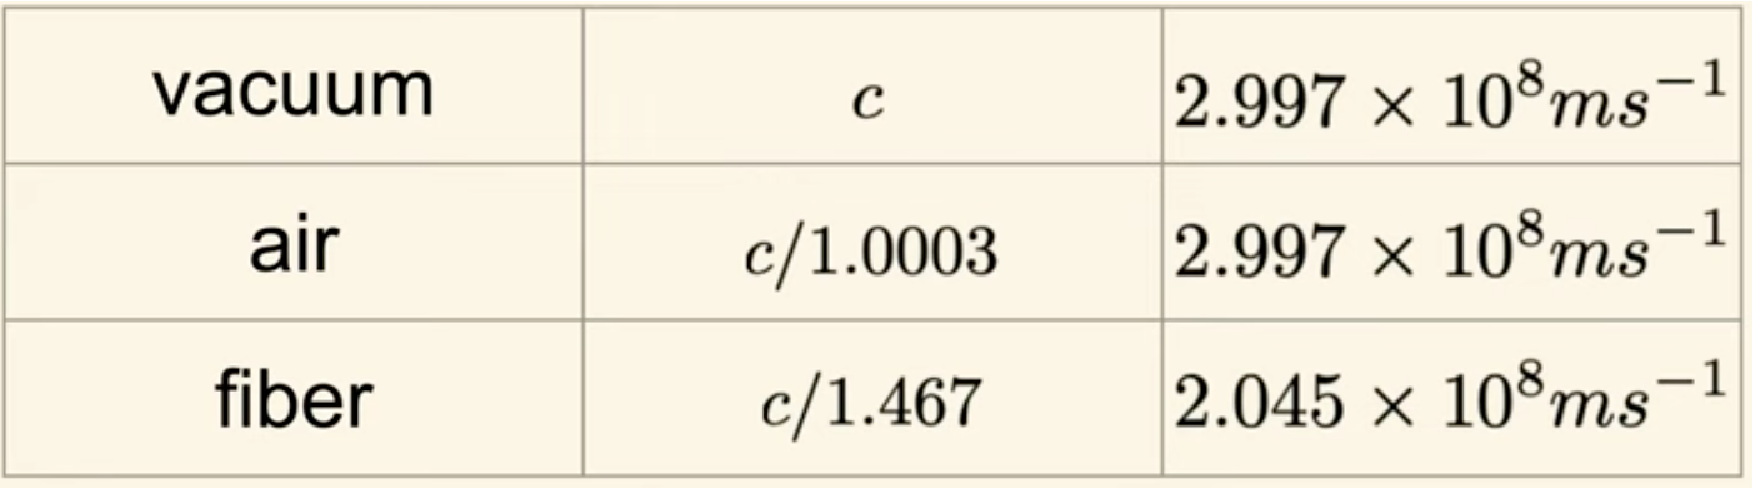
\includegraphics[width=0.9\textwidth]{lesson5/table_speeds.pdf}
    \label{図: 1}
    \caption{様々な媒質での光速}
\end{figure}
    \item 作ることが簡単です。
    \item ノイズにあまり影響を受けないこと。
\end{enumerate}
\subsection{光による通信の歴史}
光は、昔から信号として使われています。前のレッスンで説明したとおりで、万里の長城で、火から出てきた光も使っていましたし、ナポレオンのセマフォも使っていました。ちょっとだけ光ファイバーのことも説明したんですが、万里の長城とナポレオンのセマフォとしては、直行の経路が必要で、天気が良い状態でしか通信ができない。光ファイバーだったら、そういう条件はありません。
光ファイバーが世界に繋がっているんですが、下の画像は海底ケーブルの地図ですが、現代の海底ケーブルは、基本的に光ファイバーが入っているものなんですか、最初のケーブルが100年前のもので、(当時は)普通の電気の
信号が通っていたんですが、もう半世紀ぐらいは、ずっと光ファイバーでやっています:
% insert optic fibre map
\begin{figure}[H]
    \centering
    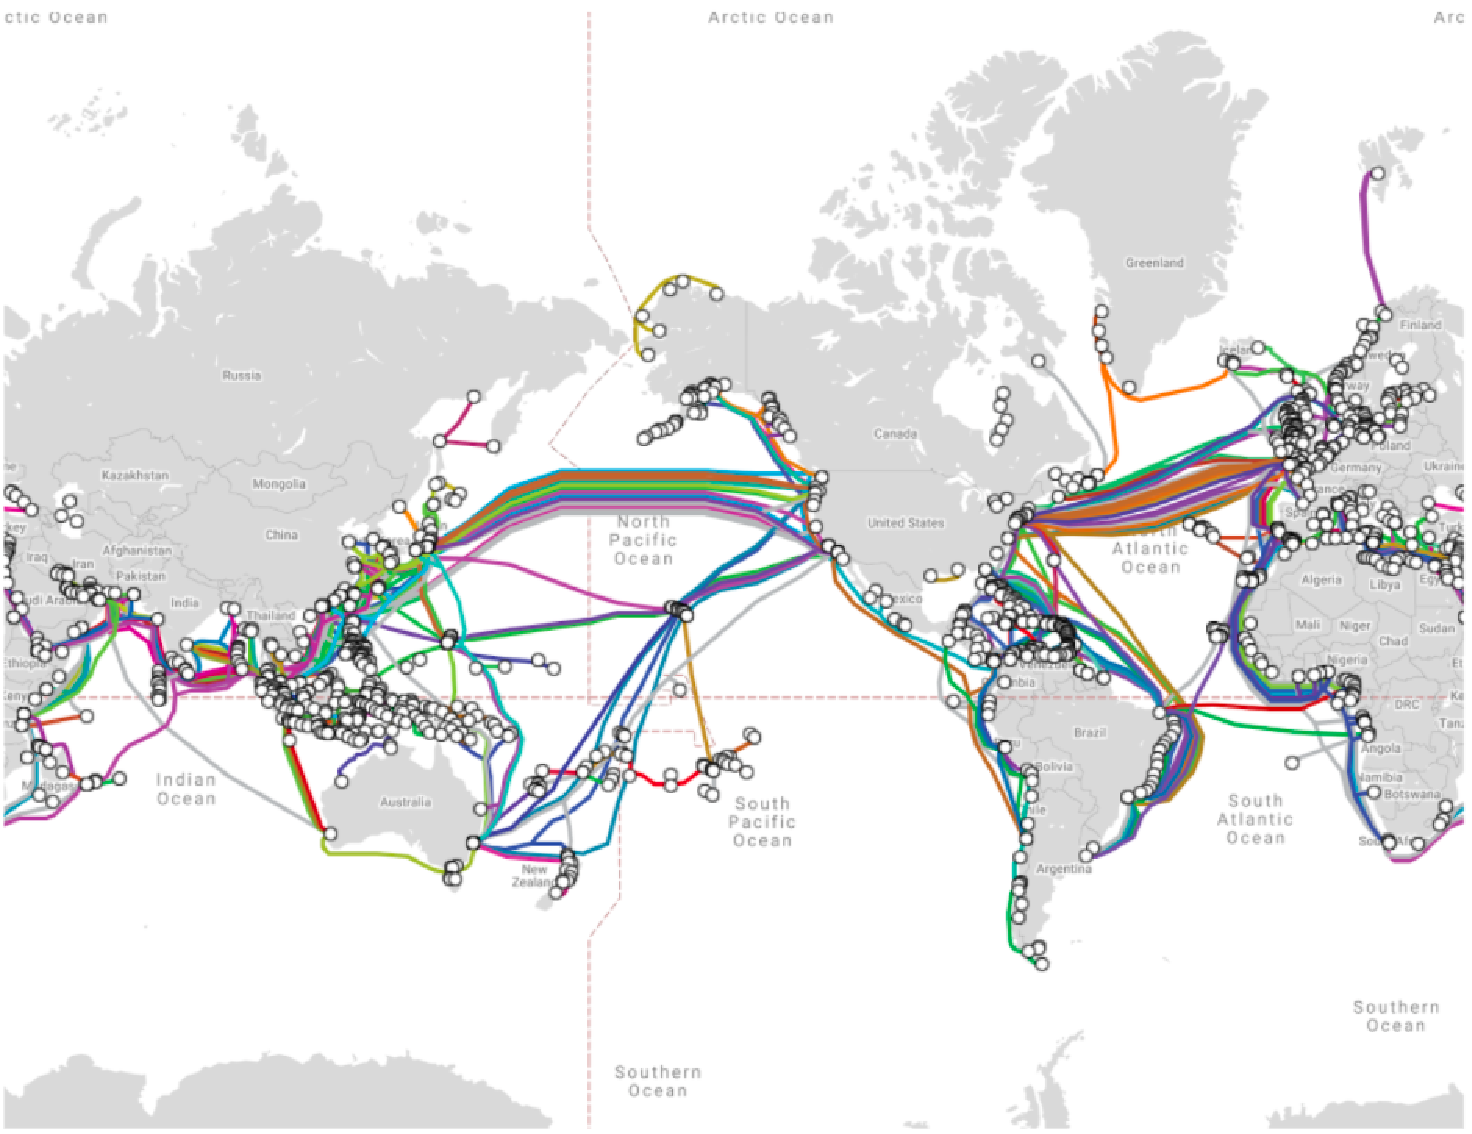
\includegraphics[width=0.9\textwidth]{lesson5/fibre_map.pdf}
    \label{図: 1}
    \caption{光学ファイバーの地図}
\end{figure}

\subsection{光の種類}
さて、光としてはどうやって区別されるのか、どうやって作るのかを見てみましょう。まずは1つの光のタイプなんですが、コヒーレントではない光:\textbf{インコヒーレントライト (Incoherent light)}なのです。普通の環境にある光は基本的にインコヒーレントな光です:
\begin{enumerate}
    \item 燃料を燃やす時などに出てくる光や、ガスが温められて出てくる
光もインコヒーレントな光です。
    \item これは簡単に作れるし、歴史的にも重要なんですが、これは基本的に古典的な光です。
\end{enumerate}
もう一つは\textbf{レーザライト(Laser light)}。
\begin{enumerate}
    \item 皆さんはレーザーという言葉を聞いたことあると思うんですが、\textit{Stimulated Emission}なんですね。
    \item Stimulated Emissionと言うのは、「誘導放出」と言う現象です。
    \item これはコーヒーレントで半世紀くらいの歴史しか持ってないんですが、今の時代としては作りやすいです。
    \item 普通の情報技術としては結構革命的な技術でした。この技術からあの新しい世界が生まれたのはレーザ光の一つの重要なポイントです。
    \item これも古典的な光ですが、これは重要で、John Dowlingという研究者がいて、彼は2020年に亡くなってしまいましたが、彼は第1回の量子革命と第2回の量子革命を説明していましたが、第1回目はトランジスターとレーザーこれがその元と言ってたんですが、現在は第2回目の量子革命ですが、これは量子コンピューターや量子通信の時代になっています。
\end{enumerate}
それから3つ目ののタイプは
\textbf{単一光子}の光\textbf{Single-photon light}なんですが、光子を一つずつ作ることです。
\begin{enumerate}
    \item 単一光子の光は作りにくいですが、色々な手法があり、1つの簡単な例は、\textbf{attenuation (減衰)}されたレーザーの光です。
    \item もう一つは、heralded光子を生成することができます。
\end{enumerate}

\section{コヒーレントな光とコヒーレントでない光}


\textit{物質はどうやって光を放出するのでしょうか?}一つの手法としては、自然な放出なんですけれども、どういうことでしょう。
\subsection{インコヒーレントな光}
% thermal excitation
\begin{figure}[H]
    \centering
    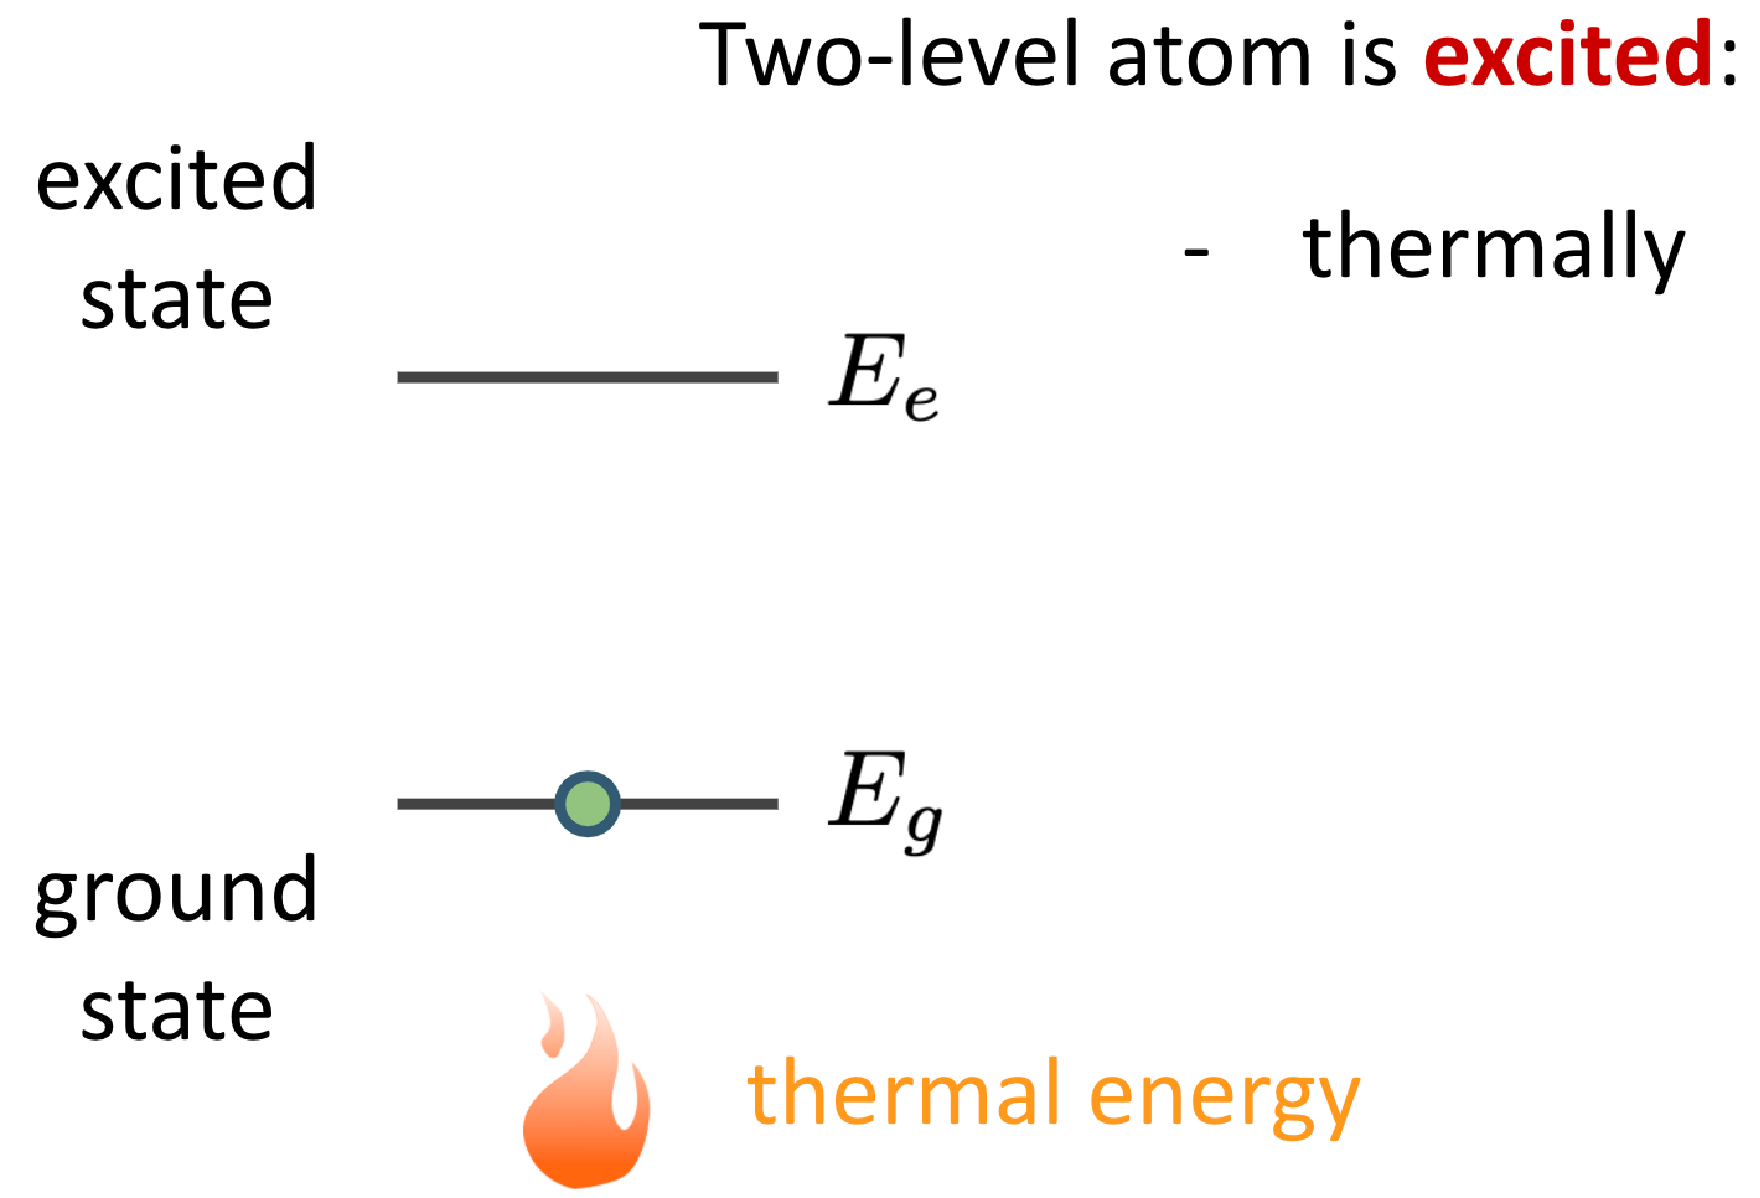
\includegraphics[width=0.9\textwidth]{lesson5/thermal.pdf}
    \label{図: 1}
    \caption{熱の励起}
\end{figure}
これはエネルギーレベルの図で、前のレクチャーで説明した通りなのですが、下の線がローレベルのエネルギーで、上の線がハイレベルのエネルギーで、それぞれ
Ground State (基底状態)と Excited State (励起状態)と言います。でこの$E_g$がGround State (基底状態)のエネルギーのレベルで、$E_e$がExcited State(励起状態)と言いいます。エネルギーが抽象的にはそれが"high level"と"low level"です。多くの原子が two levelと考えられるんですが、例えば基底状態から
他の所(状態)に行くには幾つかの方法がありますが、Excitation手法 (励起させる手法)は例えば、熱のエネルギー (Thermal energy) です。それをかけると、電子、つまりその原子の一番外側の電子のエネルギーレベルが上がり(励起状態になる)ます。もう一つの手法としてはradiation (放射)です:
% radioactive excitation
\begin{figure}[H]
    \centering
    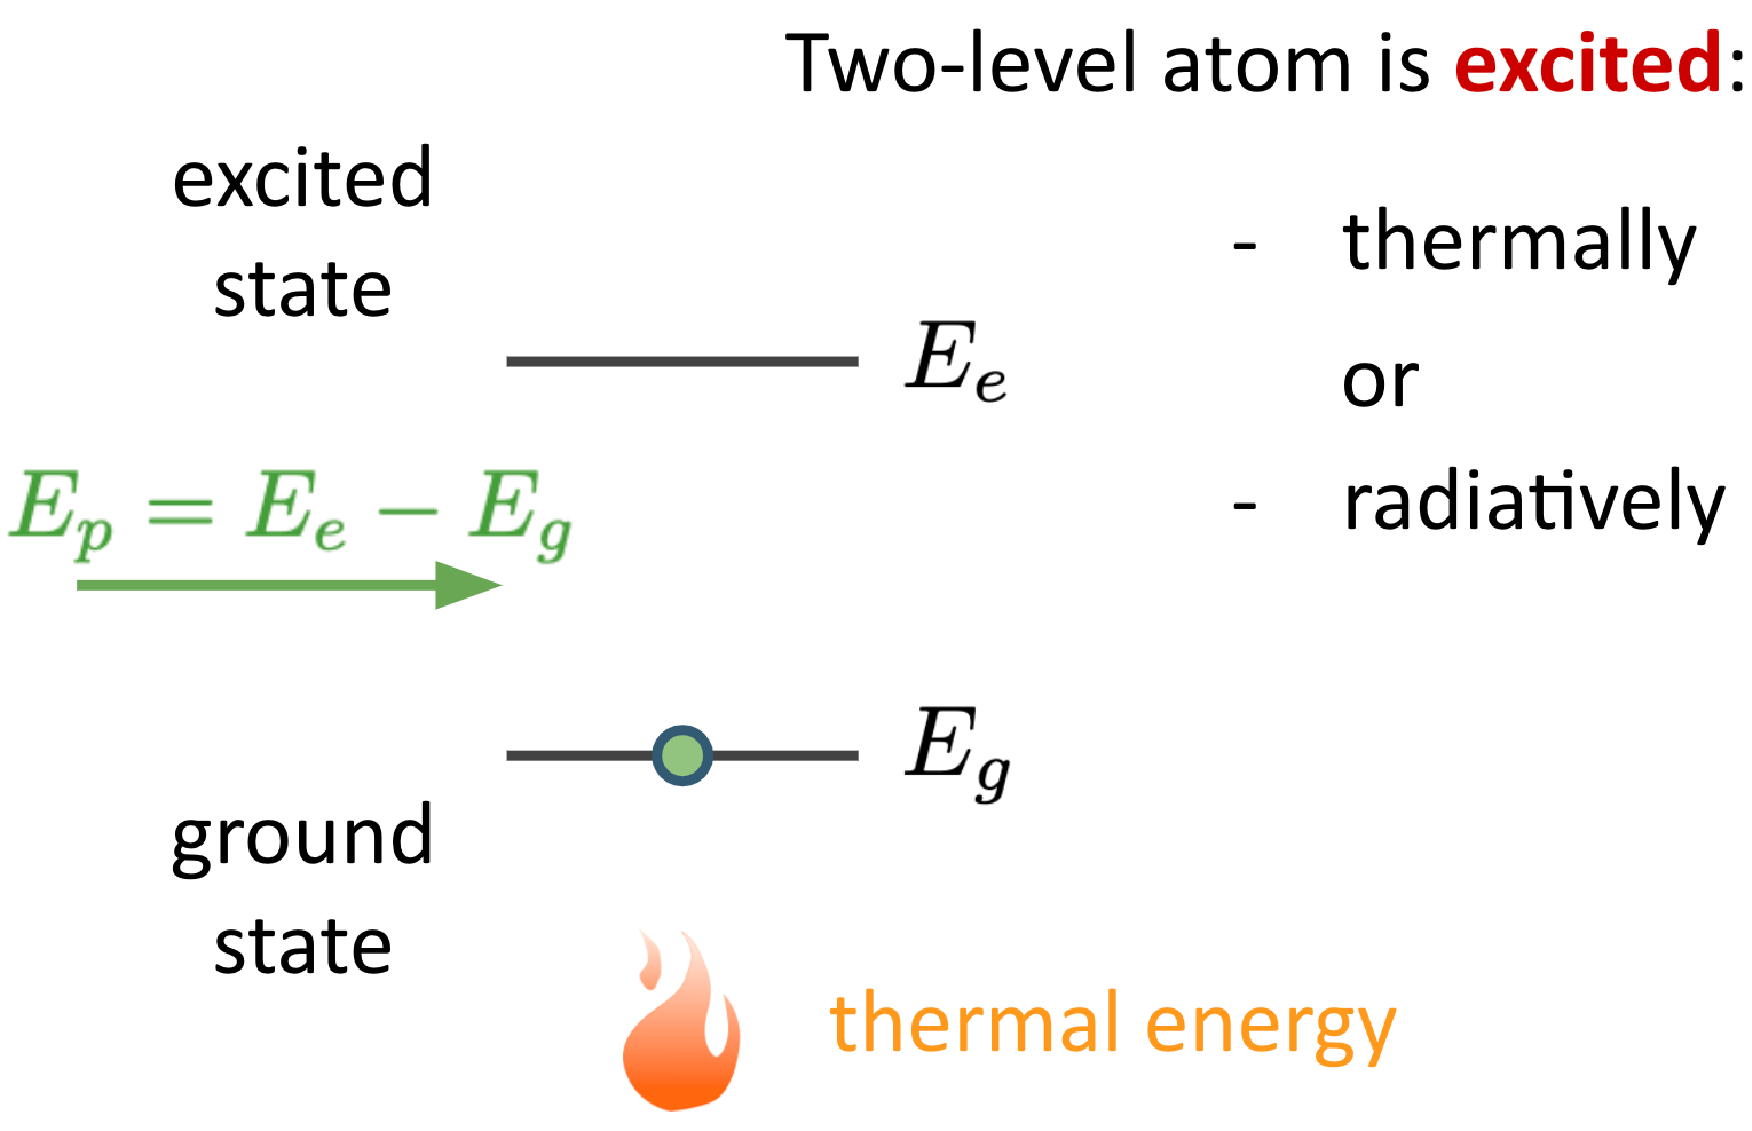
\includegraphics[width=0.9\textwidth]{lesson5/radioactive.pdf}
    \label{図: 1}
    \caption{放射の励起}
\end{figure}
Inputの光 (入力光) $E_p$というポンプの光が原子には当たるかどうか、その原子に影響するかどうかは、その原子のエネルギーのステートにはよりますけれども、$E_e-E_g$ という、この2つの(エネルギー)レベルの差が、ポンプの光のエネルギーと一緒だったら当たりやすい。

その光が原子に入ろうとすると、原子のエネルギーは上がります。しばらく経つと、いつかはspontaneous (自然的)に、上のエネルギーレベルから下のエネルギーレベルに戻ります。そのような場合には光がでてきます:
% excitation -> drop down slides
\begin{figure}[H]
    \centering
    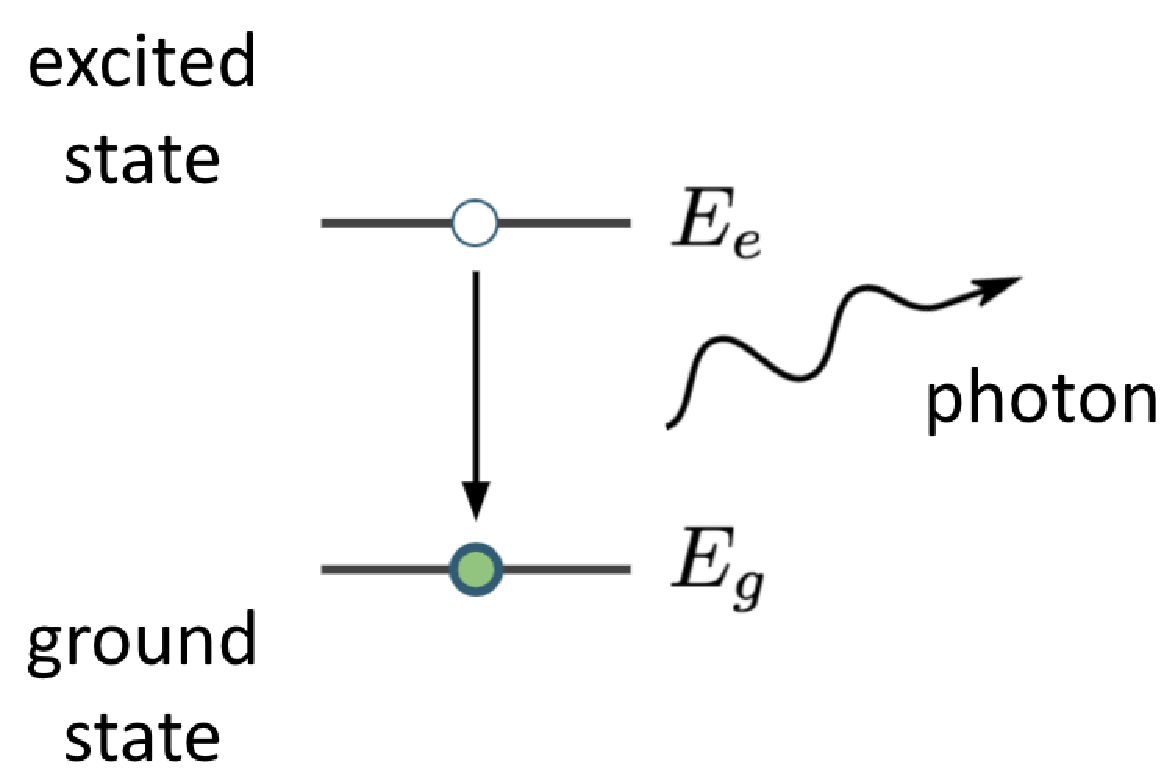
\includegraphics[width=0.9\textwidth]{lesson5/one_atom.pdf}
    \label{図: 1}
    \caption{一つの原子の自然放出}
\end{figure}
単一光子が一つが出て来ます。そして、その出てくる光子のエネルギーは$E_e-E_g$のエネルギーのレベルです。これが\textbf{Spontaneous Emission (自然放出)}です。

それが一つの原子なんですけれども、これが例えば、二つの原子がある場合には、二つともそのExcited(励起)の状態から始まると、各原子がいつかはspontaneousに落ちてくるのですが、その時には、各原子から単一光子が一つずつ出てきます:
% two different atoms
\begin{figure}[H]
    \centering
    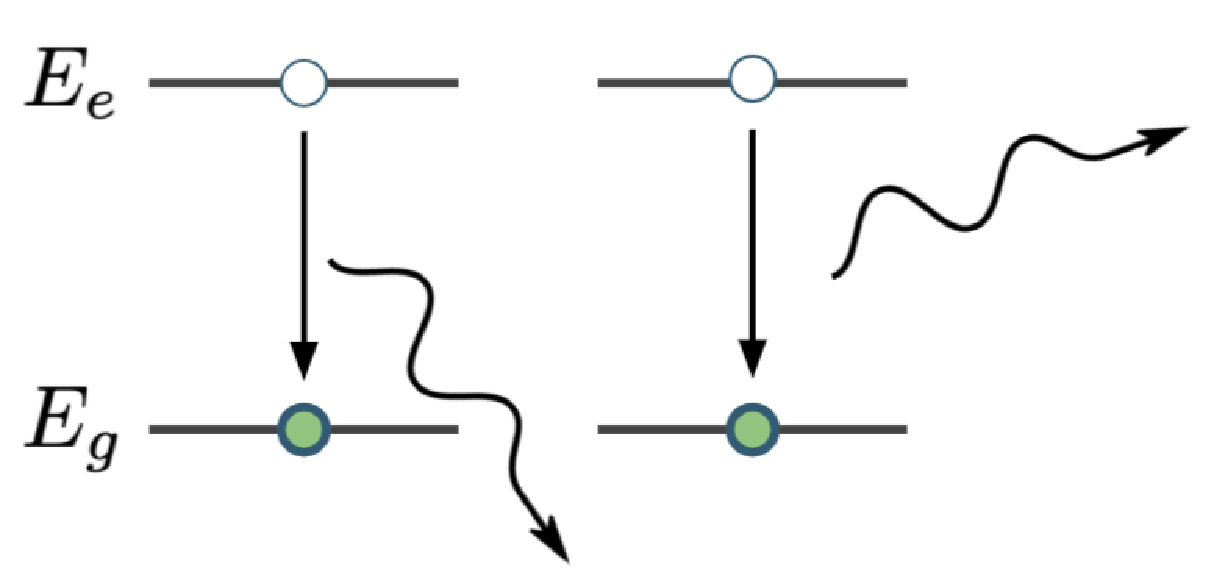
\includegraphics[width=0.9\textwidth]{lesson5/two_atoms.pdf}
    \label{図: 1}
    \caption{二つの原子の自然放出}
\end{figure}
タイミング等は基本的に独立なので、\textit{位相も違うし}、\textit{出てくる方向も違う}し、基本的にこれらは独立な光になっています。それらが\textbf{インコヒーレントな状態}といいます。

そのような原子がいっぱいある場合、例えばこれが普通の古い手法の、電球なんですがそういう電球から出てくる光は容量は出てきますが、電球の中には、針金があるんですが、その針金に電流を流して、その電流が熱になって、その針金が熱くなって、針金の各原子が励起状態になるんですが、その励起状態から基底状態に戻る場合には、各原子から光子も出てきます:
% lightbulb
\begin{figure}[H]
    \centering
    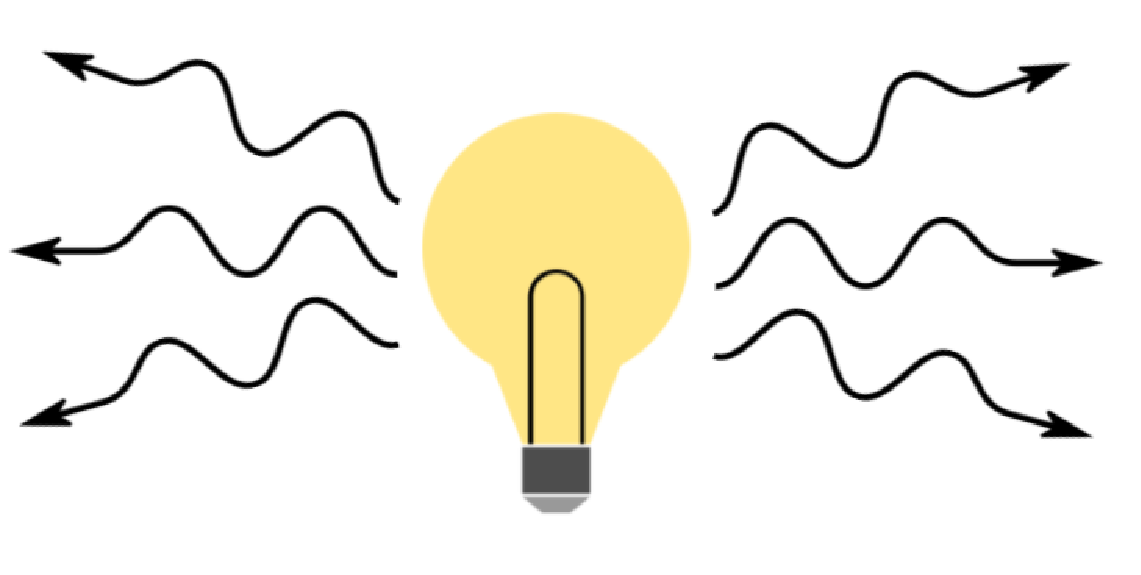
\includegraphics[width=0.9\textwidth]{lesson5/lightbulb.pdf}
    \label{図: 1}
    \caption{電球(インコヒーレント)}
\end{figure}
その場合には、(光子の)エネルギーのレベルや、位相がそれぞれ異なる場合もありますからそれらは基本的にインコヒーレントです。コヒーレントがない状態の光は\textbf{周波数}、\textbf{波長}も違いますし、\textbf{方向}、\textbf{位相}も違うんです。

\subsection{コヒーレントな光}
そうするとコヒーレントの状態とはどう違うのでしょう?いくつかの特別な特徴があるんですけれども、重要なポイントは、周波数が一つしかなく、つまり色も一つしかないです:\textbf{(monochromatic)}あとは方向も一緒で、位相も揃っています。
そうすると、これがコヒーレントな状態になります。光はいくつかの光子がいっぱい一緒に出てくると、 これが\textbf{Coherent light source}になると思います。そうするとこれがどのようなsourceになるのかを次のステップで説明します。


\section{レーザー 1}
さっきのステップではコヒーレントな光はどうやって作られると言う話をしていたんですが下の図がありましたよね:
% laser placeholder "[????]"
\begin{figure}[H]
    \centering
    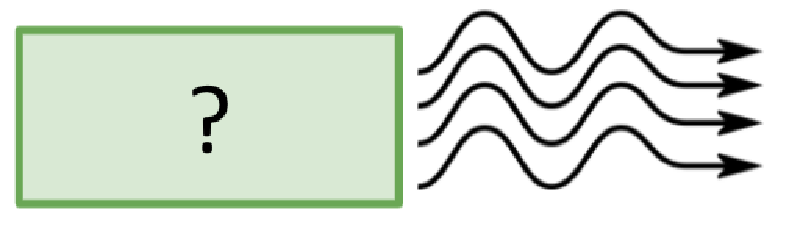
\includegraphics[width=0.9\textwidth]{lesson5/question_box.pdf}
    \label{図: 1}
    \caption{箱には「????」}
\end{figure}

多分皆さんがわかっていると思うんですけれども、この箱は何でしょう? レーザーですよね。
% laser box
\begin{figure}[H]
    \centering
    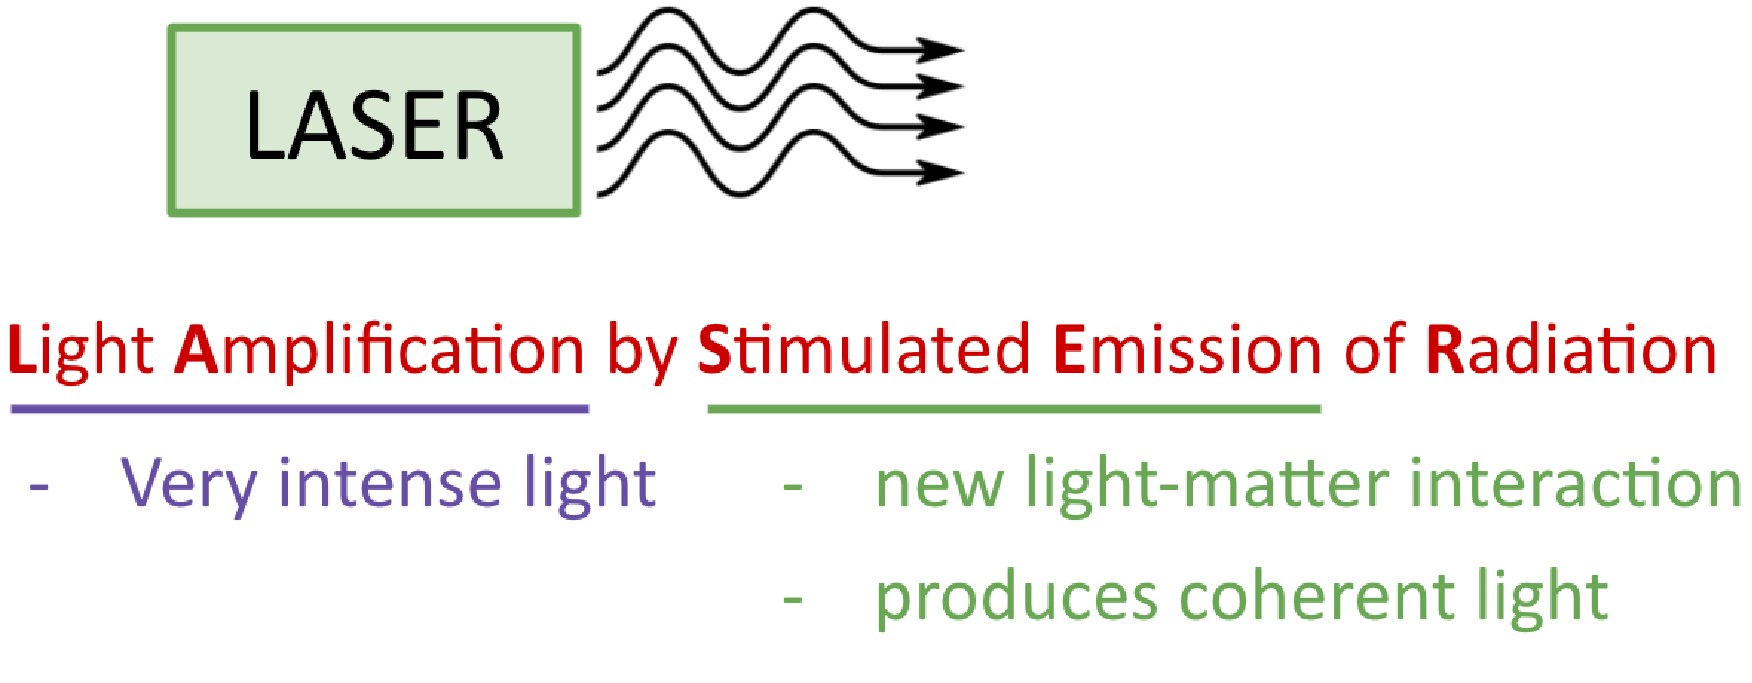
\includegraphics[width=0.9\textwidth]{lesson5/LASER_box.pdf}
    \label{図: 1}
    \caption{LASERでした}
\end{figure}
説明するんですけれども、このステップは長いので、ちょっと我慢して進みましょう。レーザーと言うのは、ただの言葉ではなく、acronym (頭文字)abbreviation (略語)ですが、\textbf{L}ight \textbf{A}mplification by \textbf{S}timulated \textbf{E}mission of \textbf{R}adiation (LASER).
"Stimulated Emission"というのが誘導放出で、光物質相互作用といい、Light (光)と Matter (物質)の相互作用です。これによってコヒーレントな光を作れるんですね。この"Light Amplification"(増幅)の場合にはこれがだんだん光は強くなることでしょう。
\subsection{三つの光と物質相互作用}

この光物質相互作用では、基本的に3つのことが重要なんですが、これがエネルギーレベル図で、一つの原子がExcited(励起)の状態になっていて、それが基底状態に落ちることが一つ目なんですが、こういう場合には(単一の)光子が出てきますよね。これが\textbf{Spontaneous Emission}(自然放出)です:
% spontaneous emission
\begin{figure}[H]
    \centering
    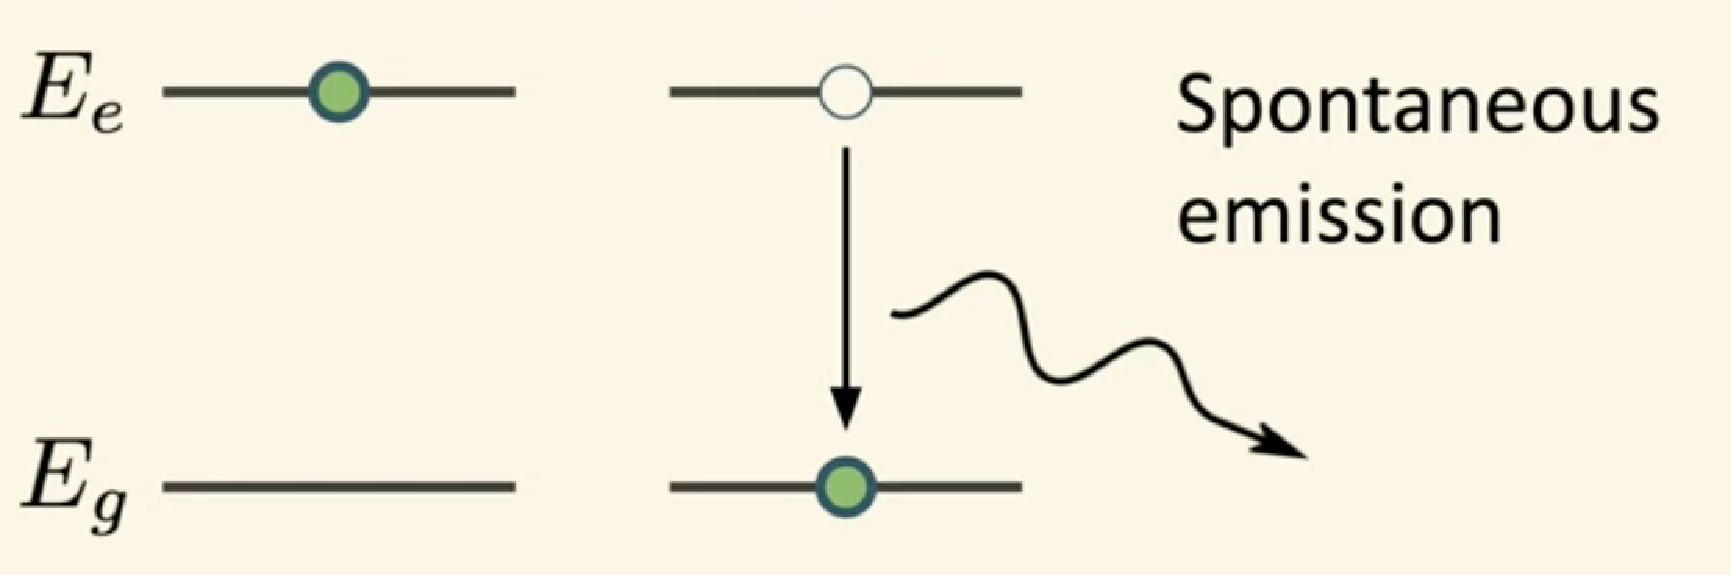
\includegraphics[width=0.9\textwidth]{lesson5/spontaneous_emission.pdf}
    \label{図: 1}
    \caption{自然放出}
\end{figure}


二つ目なんですが、基底状態から始まって、光が入ってくると、エネルギーレベルが上ってきて、基底状態から励起状態になることを、\textbf{Stimulated Absorption (誘導吸収)} といいます:
% stimulated absorption
\begin{figure}[H]
    \centering
    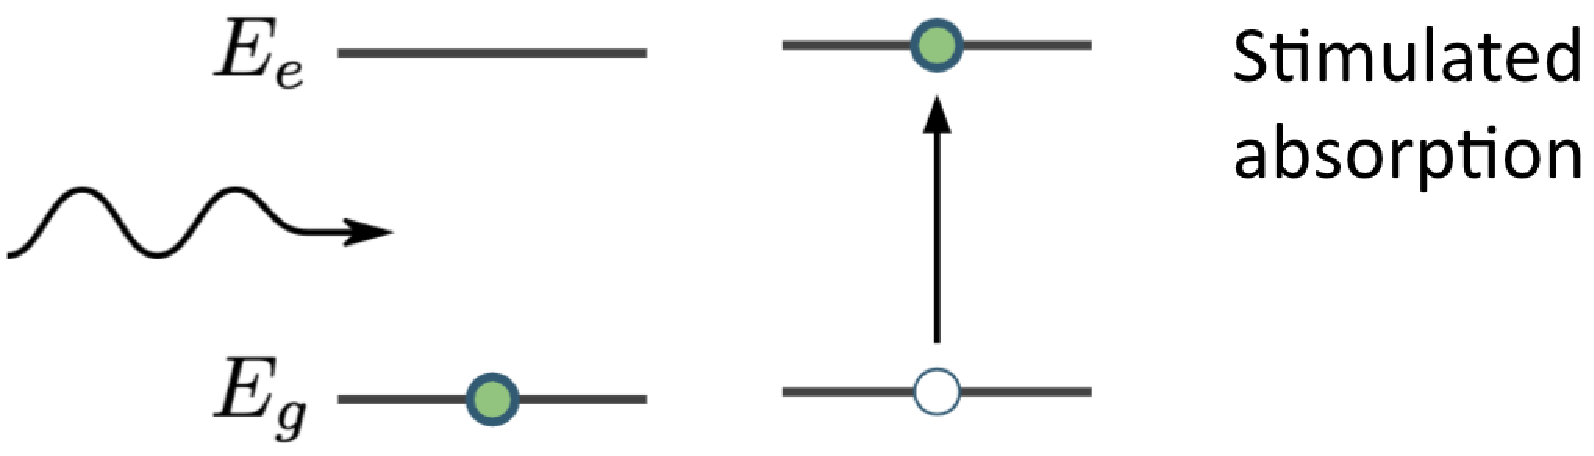
\includegraphics[width=0.9\textwidth]{lesson5/stimulated_absorption.pdf}
    \label{図: 1}
    \caption{誘導吸収}
\end{figure}

三つ目は、光が入ってきて、原子が励起状態ですが、最初の光が通るんですが、それが直接原子にはAbsorption(吸収)されず、その光が通ると待ってた原子が、励起状態から基底状態に戻ることがあり、それも光子出てきますから、最初に一つの光子が入って、最後には2つ(の光子)が出てきますね。インプットは一つの光子でアウトプットは2つの光子になります。これはStimulated Emission (誘導放出)です:
% Stimulated Emissions
\begin{figure}[H]
    \centering
    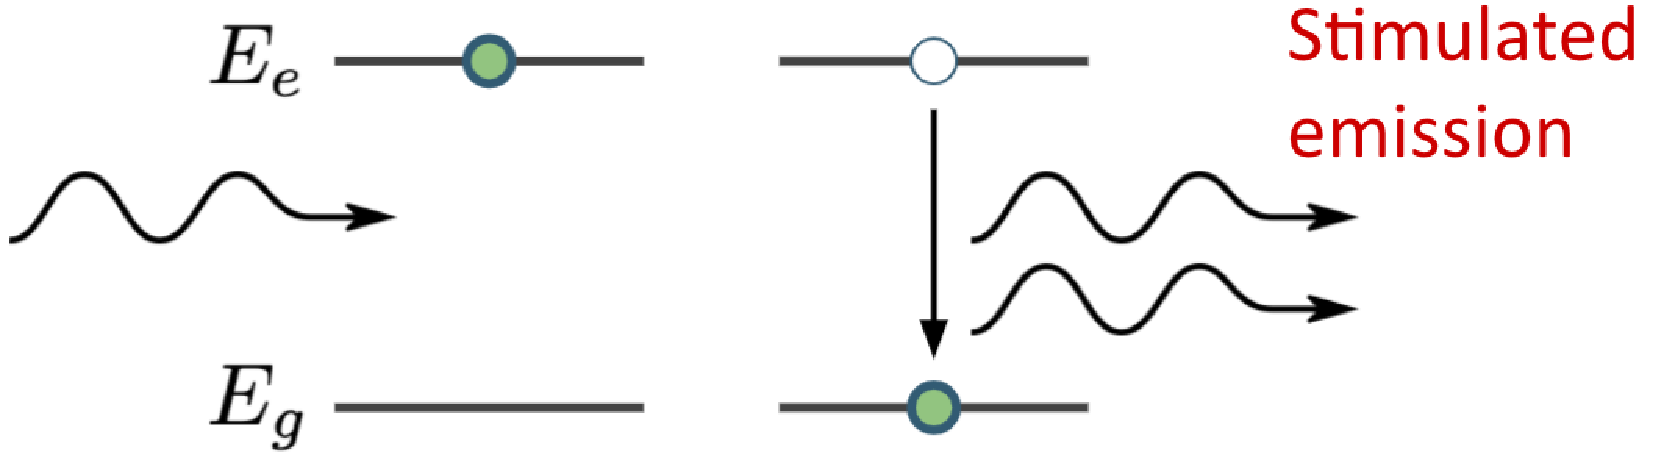
\includegraphics[width=0.9\textwidth]{lesson5/stimulated_emission.pdf}
    \label{図: 1}
    \caption{誘導放出}
\end{figure}

誘導放出の場合、\textbf{周波数は一緒}ですし、\textbf{方向も同じ}ですし
\textbf{位相も揃っています}。これによって、この光はコヒーレントな状態といいます。Polarization(偏光)も一緒になりますが、この場合にはあまり重要ではないです。

\subsection{増幅(Amplification)}
誘導放出はAmplification(増幅)にもなるんですが、インプットの光とアウトプットの光で、Amplificationの場合には、アウトプットの光が強くなることをいいます:
% expontentially increasing photons
\begin{figure}[H]
    \centering
    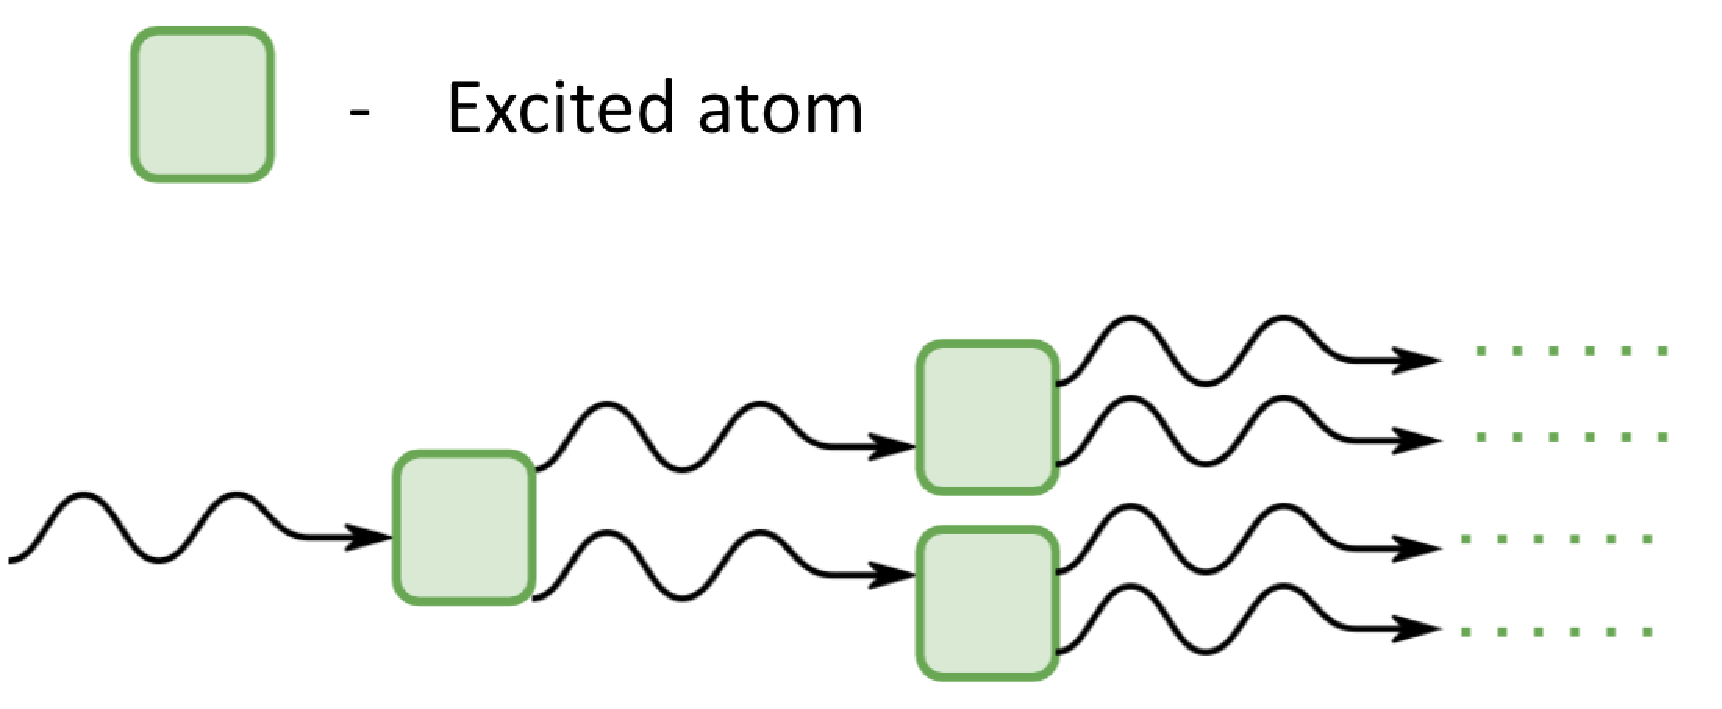
\includegraphics[width=0.9\textwidth]{lesson5/exponential_photons.pdf}
    \label{図: 1}
    \caption{光子の指数的な関数}
\end{figure}
そうすると、ExcitedなAtom(励起状態の原子)は光を、その原子に通して、もっと強い光が出てくることになります。一つから二つになって、二つから四つになるような指数的な関数で現れる場合もあります。

\textit{問題は、すべての原子は励起状態にはなってない}から、どうやってその励起状態を作るとか、どうやってそれを使うのかが、レーザーのデザインの一番重要なポイントです。
\subsection{反転分布}
数えてみましょう:
% "Accounting Table"
\begin{figure}[H]
    \centering
    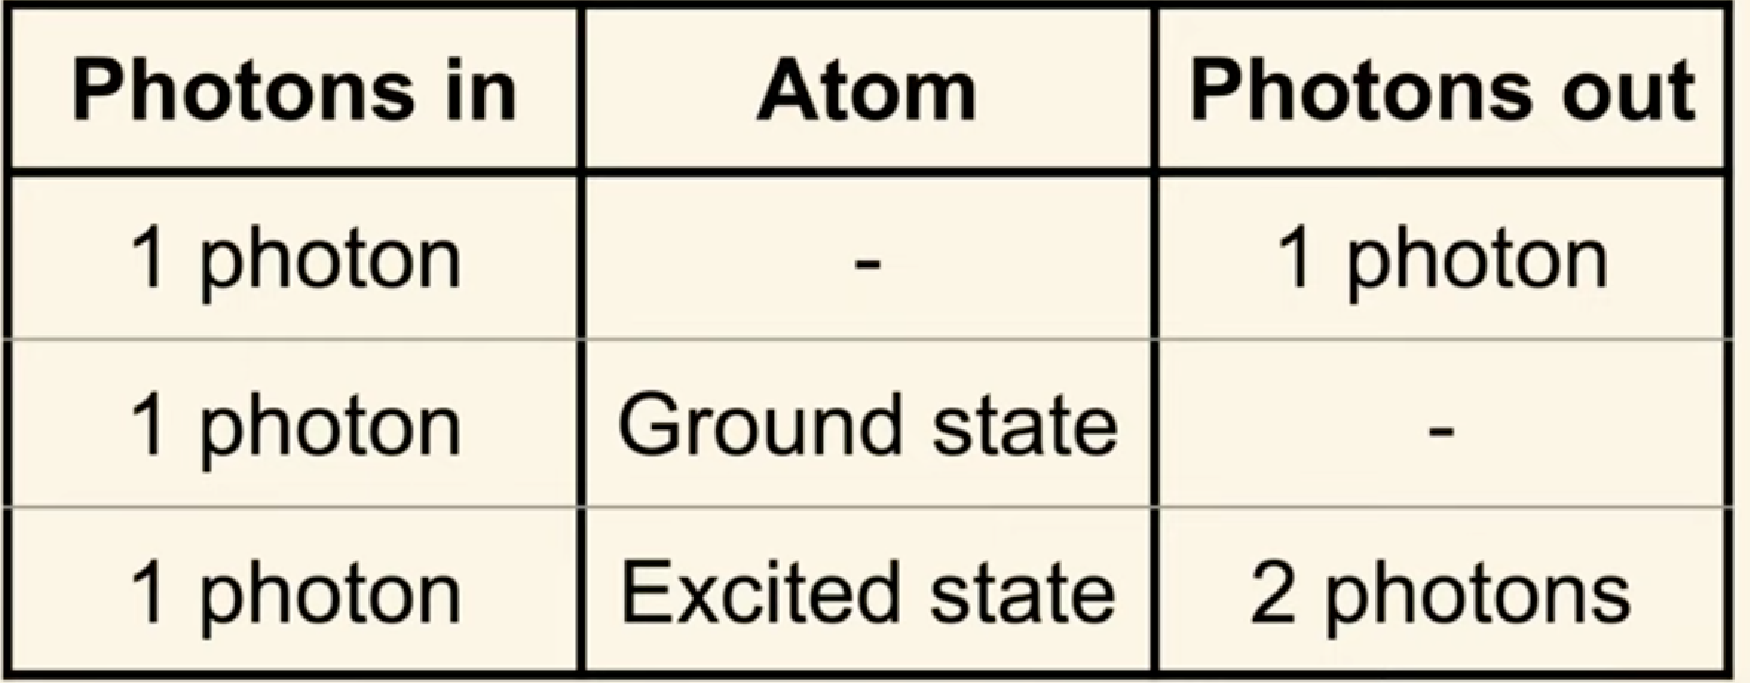
\includegraphics[width=0.9\textwidth]{lesson5/photon_table.pdf}
    \label{図: 1}
    \caption{単一光子の表}
\end{figure}
この表は単一の光子を一つ入れて、それが原子の状態によって出てくる光子の状態を表しています。
\begin{itemize}
    \item 一番多いのは、光は入ってきますが、原子には当たらず影響が無い場合で、それがインプットは一つの光子で、アウトプットは一つの光子なので、状態はあまり変わりません。
    \item もう一つのやり方として、一つの光子入れて、当たる原子が基底状態の場合は、光子が誘導吸収によってアウトプットは0個の光子になります。インプットとは一つで、アウトプットが0なので、光の強さは下がります。
    \item もう一つとしては、一つの光子をインプットして当たる原子が励起状態になっている場合にはアウトプットの光子は2つになりますね。これが誘導放出で、光は強くなります。これは光子の数が変わります。
\end{itemize}

もう少し具体的な例を見てみると、例えば4つの原子を使いましょう:
% 4 ground
\begin{figure}[H]
    \centering
    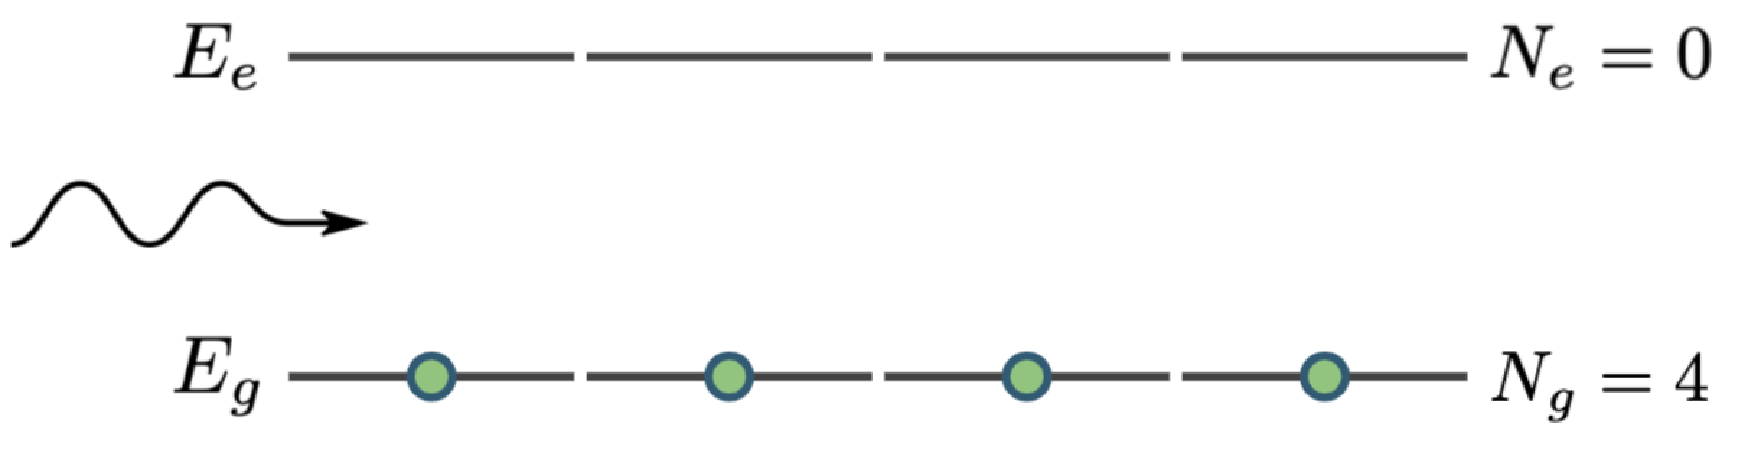
\includegraphics[width=0.9\textwidth]{lesson5/4_ground.pdf}
    \label{図: 1}
    \caption{4基底状態・0励起状態}
\end{figure}
$E_g$はGround Stateといい、基底状態にある原子で、$E_e$は励起状態  (Excited State)といい、初期状態は4つとも基底状態になっているんですね。光が入ってきて、さっきの3つの光物質相互作用には、3つの選択肢があったんですけど、何も影響がないというのと、誘導放出と誘導吸収です。今回の場合は放出はないですよね。Excited State(励起状態)がないので。\textbf{誘導吸収にしかなりません}
% 3 ground 1 excited
\begin{figure}[H]
    \centering
    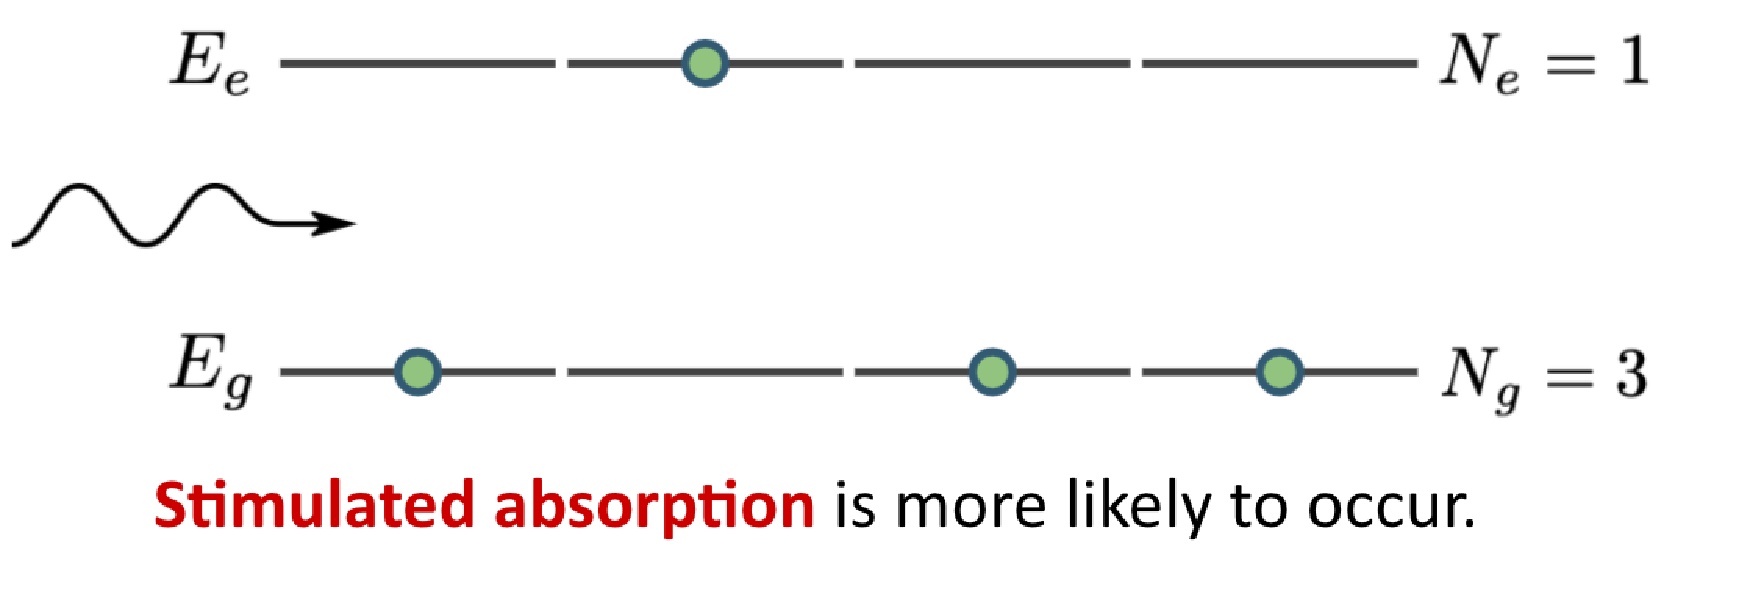
\includegraphics[width=0.9\textwidth]{lesson5/3_ground_1_excited.pdf}
    \label{図: 1}
    \caption{3基底状態・1励起状態}
\end{figure}
例えば2つ目の原子が(光子を)吸収して、残りの3つの(原子の)状態は基底状態になり、1つは励起状態になります。もう一つの光子が入ってくる場合は、確率的なことが起こります。今は3つの原子が基底状態で、1つは励起状態なので、\textbf{確率的には放出ではなくて、吸収の場合が多いです}。
% 2 ground/excited
\begin{figure}[H]
    \centering
    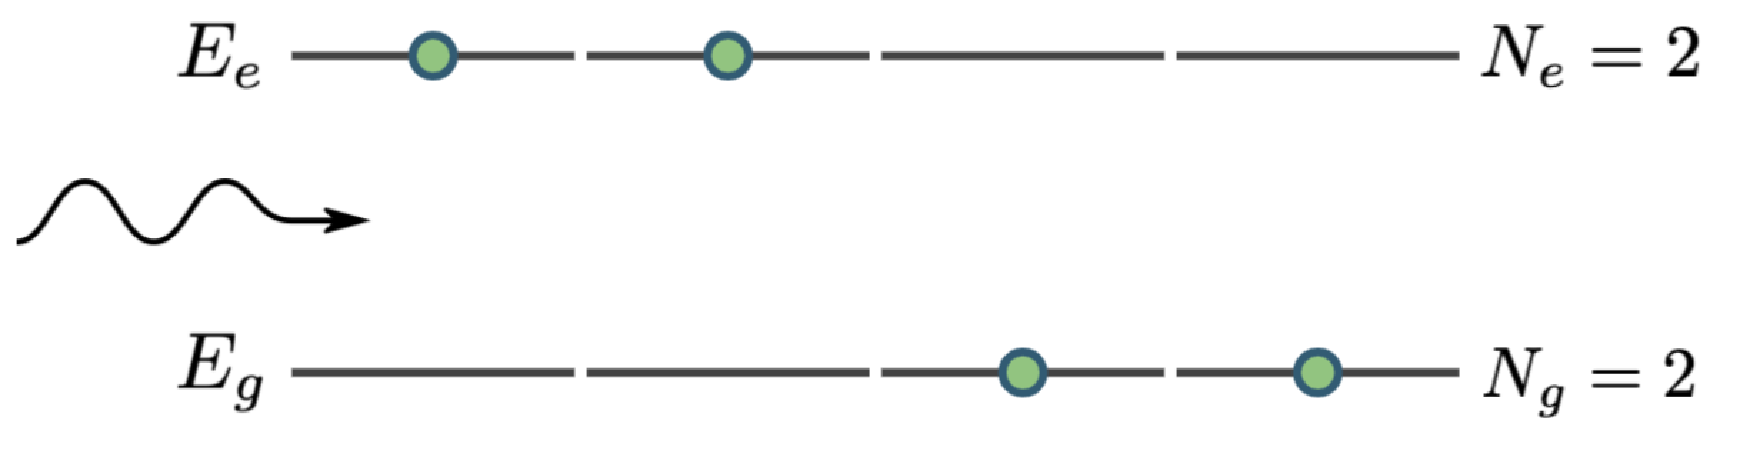
\includegraphics[width=0.9\textwidth]{lesson5/2_ground_2_excited.pdf}
    \label{図: 1}
    \caption{2基底状態・2励起状態}
\end{figure}
そうすると1つ目(の原子)が上がる(励起する)ことになります。3つ目の光子が入ってくると、この場合は50:50です。励起状態と基底状態(の原子の数)は一緒なので、\textbf{確率的には一緒}なんですが、光の強さは確率的、統計的にはあまり変わらないです。

この場合、(光子の)吸収はどうなるでしょうか?この場合、3:1になっているため、次のステップとしては、\textbf{放出(が起こる)の方が確率は高い}です。
\begin{figure}[H]
    \centering
    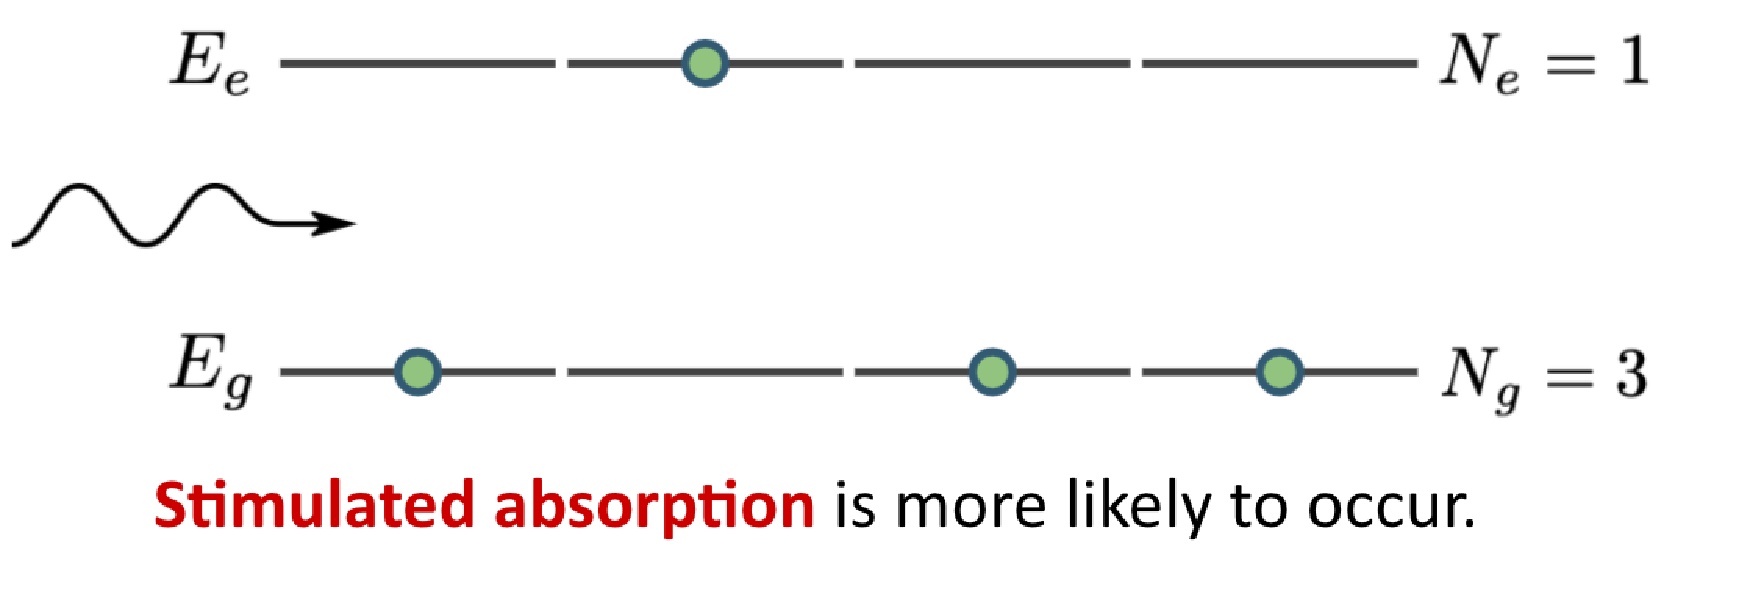
\includegraphics[width=0.9\textwidth]{lesson5/3_ground_1_excited.pdf}
    \label{図: 1}
    \caption{1基底状態・3励起状態}
\end{figure}
誘導放出になる場合には、それがどういう状態が統計的には多いのか$N_e$の数が$N_g$の数より多い場合を\textbf{population inversion(反転分布)}といいます。(その場合には)多くの原子がExcited State(励起状態)になっています。一つ重要な問題あるんですけれども、
$N_g$が$N_e$より多い場合には、$N_e$は増え、$N_e$が多い場合には、$N_g$が増える:

$N_{g}>N_{e} \implies N_{e}$ 増加

$N_{g}<N_{e} \implies N_{g}$ 増加 

それが連続すると、最終的には\textbf{$N_g=N_e$}になって、入れている光と出てくる光の強さは一緒になります。
この中で反転分布はどのように作るのでしょう?一つの基本的な概念としては、さっきまでは2 levelのシステムの話をしてたんですけれども、基底状態と励起状態は1つずつ(のエネルギーレベル)を使っていたんですが、(エネルギーレベルが)3つの状態の原子を使うと、反転分布をもっと簡単に作れます。それは次のステップで説明します。


\section{レーザー 2}
\subsection{三つのエネルギーレベルの原子モデル}
2つのエネルギーレベルではなく、3つのエネルギーレベルを使うことが必要だという話をしましたが、どのようにやるのかを見ていきましょう。これは反転分布を作るためです:
% 3 level atom, annotated
\begin{figure}[H]
    \centering
    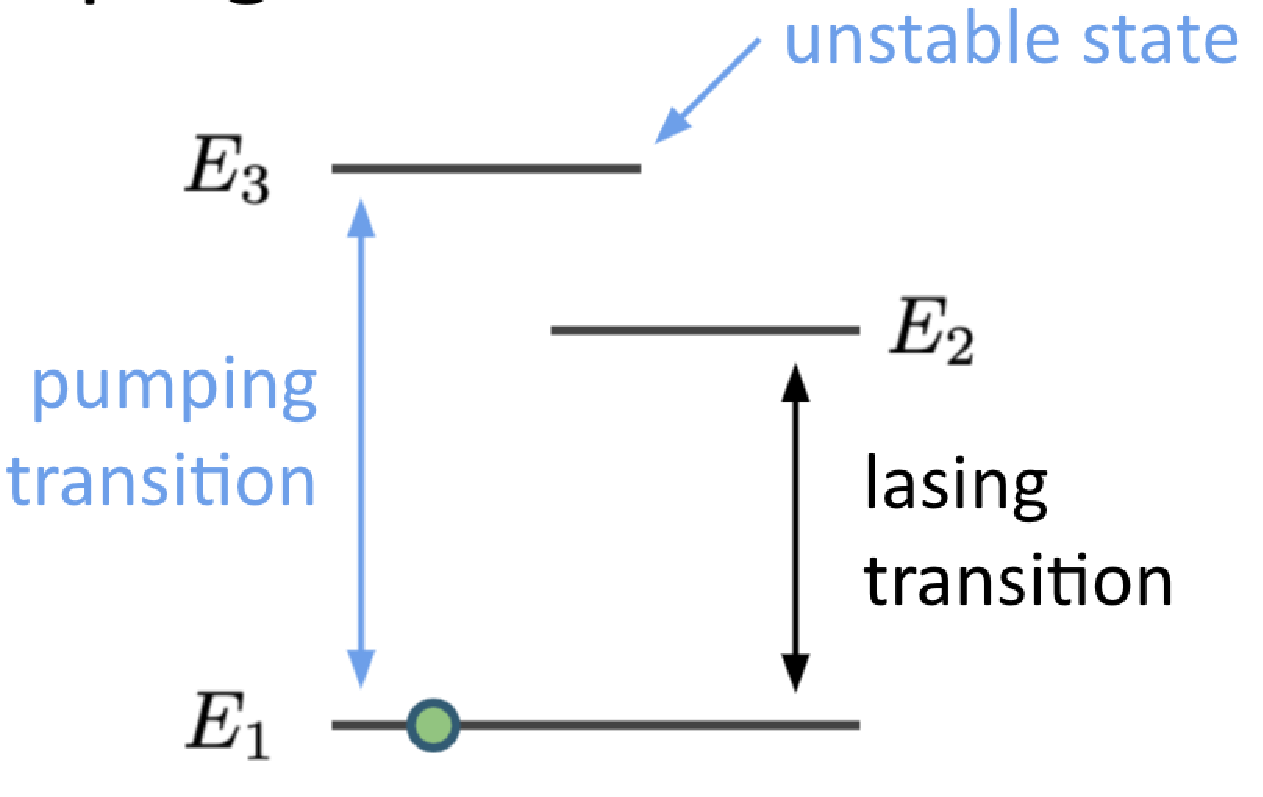
\includegraphics[width=0.9\textwidth]{lesson5/3_atom_annotated.pdf}
    \label{図: 1}
    \caption{三つのエネルギーレベルの原子モデル}
\end{figure}
前の例では$E_g$(基底状態)と$E_e$(励起状態)と言っていましたが、今回は3つのレベルの状態を使います。$E_1$, $E_2$, $E_3$とあって、$E_3$が最もエネルギーが高い状態です。この場合$E_3$は不安定な状態です。$E_1$から$E_3$にエネルギーが上がることを、\textbf{pumping transition}と言います。$E_2$から$E_1$に戻る場合は\textbf{lasing transition}と言います。ではどのように使うのでしょうか。
% 3 atom stage 1 [incoming photon]
\begin{figure}[H]
    \centering
    \includegraphics[width=0.5\textwidth]{lesson5/stag$E_1$.pdf}
    \label{図: 1}
    \caption{ポンプステージ1}
\end{figure}
青い矢印がポンプの光で、この光のエネルギーは、$E_3$と$E_1$のエネルギーレベルの差と等しく設定しています。そうすると、原子のエネルギーレベルは$E_1$から$E_3$へ上がります:
% stage 2 [up to $E_3$]
\begin{figure}[H]
    \centering
    \includegraphics[width=0.5\textwidth]{lesson5/stag$E_2$.pdf}
    \label{図: 1}
    \caption{ポンプステージ2}
\end{figure}

これ($E_3$)が不安定な状態なので、いつか変わってしまうのですが、laser transitionには影響しません。不安定な状態のため、自然にエネルギーレベルが$E_3$から$E_2$に落ちます:
% stage 3 [$E_2$]
\begin{figure}[H]
    \centering
    \includegraphics[width=0.5\textwidth]{lesson5/stag$E_3$.pdf}
    \label{図: 1}
    \caption{ポンプステージ3}
\end{figure}

laserの物質の結合にエネルギーが転送され、最終的には熱に変換され、原子の振動等に影響します。少しのエネルギーがそのように転送され、(エネルギーレベルが)$E_3$から$E_2$へ減衰します。そうすると$E_2$から$E_1$への転移の準備ができたことになります。これを使って誘導放出を起こしたいとします。その時、もう一つの光子のエネルギーを$E_2$と$E_1$のエネルギーの差に合わせて入れると、一つの光子が入力になり、(誘導放出が起こり)二つの光子が出力になります:
% stage 4/5 [Stimulated emission before/after]
\begin{figure}[H]
  \centering
  \begin{minipage}[b]{0.4\textwidth}
    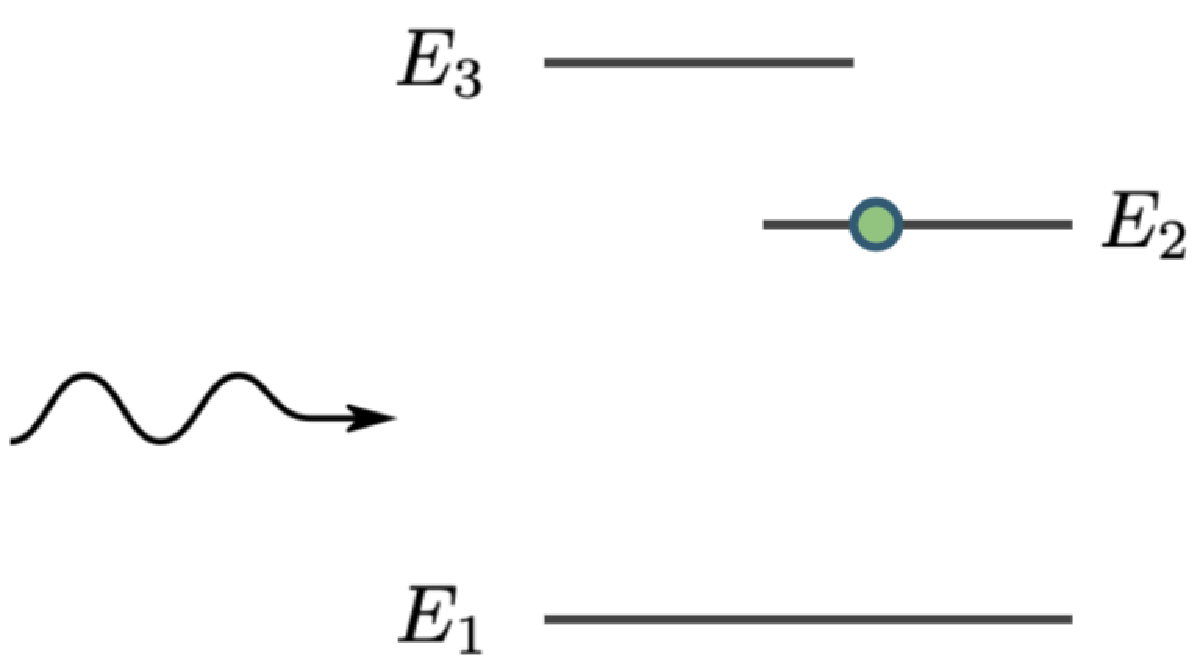
\includegraphics[width=\textwidth]{lesson5/stage4.pdf}
    \caption{ポンプステージ4}
  \end{minipage}
  \hfill
  \begin{minipage}[b]{0.4\textwidth}
    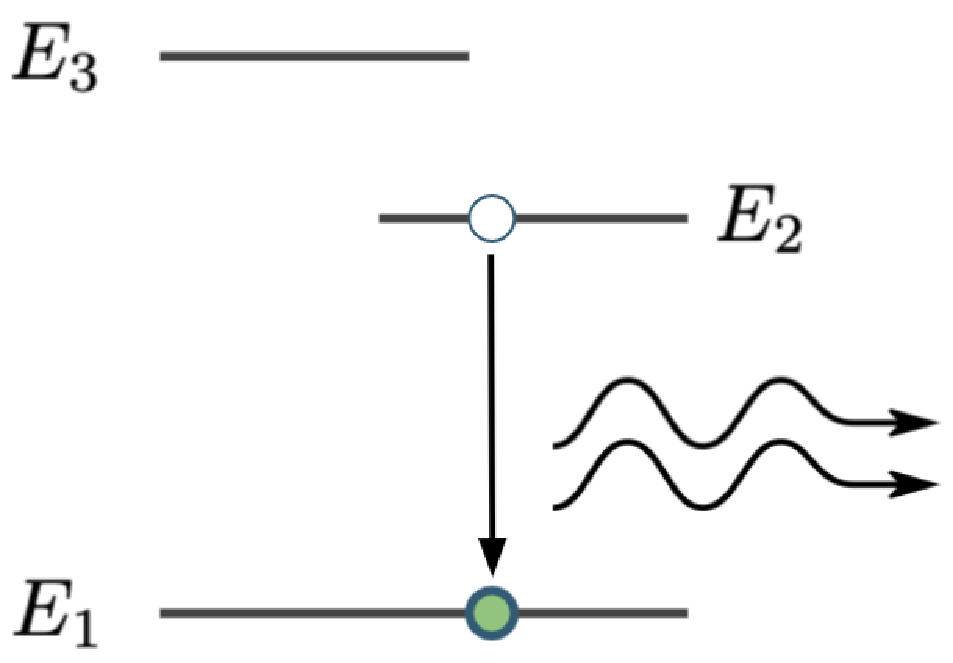
\includegraphics[width=\textwidth]{lesson5/stage5.pdf}
    \caption{ポンプステージ5}
  \end{minipage}
\end{figure}
この場合は光の大きさが強くなる(増幅)になります。通常は、同時にpumping lightとインプットのレーザーの光を同時に入れて、pumping lightが$E_1$のエネルギーレベルにある原子のエネルギーを$E_3$に上げて、自然に$E_2$に落ちて、レーザーの一つのインプットの光子は二つのアウトプットの光子になります。そうするとこれはAmplification(増幅)になります。
これを連続的に行い、pumping lightの効率が良ければ、多くの原子が$E_3$の状態にあるので、安定的にこのプロセスを続けることができます。これは反転分布になっていて、$N_1$, $N_2$はGround StateとExcited stateの原子の数になっています: $N_2$ > $N_1$
\pagebreak
\subsection{レーザーの構造}

レーザーの内部は、様々な材料(液体や気体等)で作ることが可能で、それらをレーザーの\textbf{利得媒質 (gain medium)}と言いますが、それらを使って光の強さを増幅したいとします:
% medium, random direction photons
\begin{figure}[H]
    \centering
    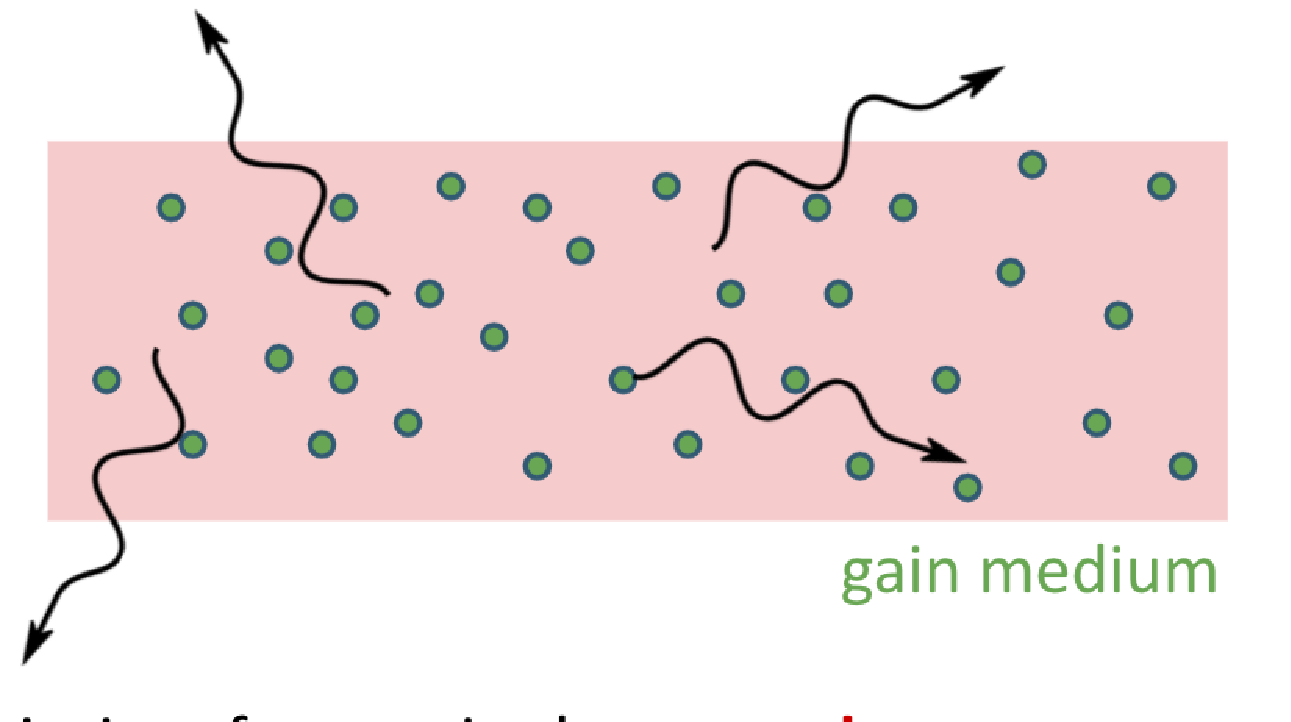
\includegraphics[width=0.5\textwidth]{lesson5/medium_random.pdf}
    \label{図: 1}
    \caption{利得媒質}
\end{figure}
最初は多くの原子が基底状態で、出てくる光は\textbf{Spontaneous Emission (自然放出)}です。\textbf{どのようなものでも、絶対零度でなければ光は出てきます。}我々が行いたいのは、媒質をポンプの状態(励起状態)にすることです:
% medium + pump
\begin{figure}[H]
    \centering
    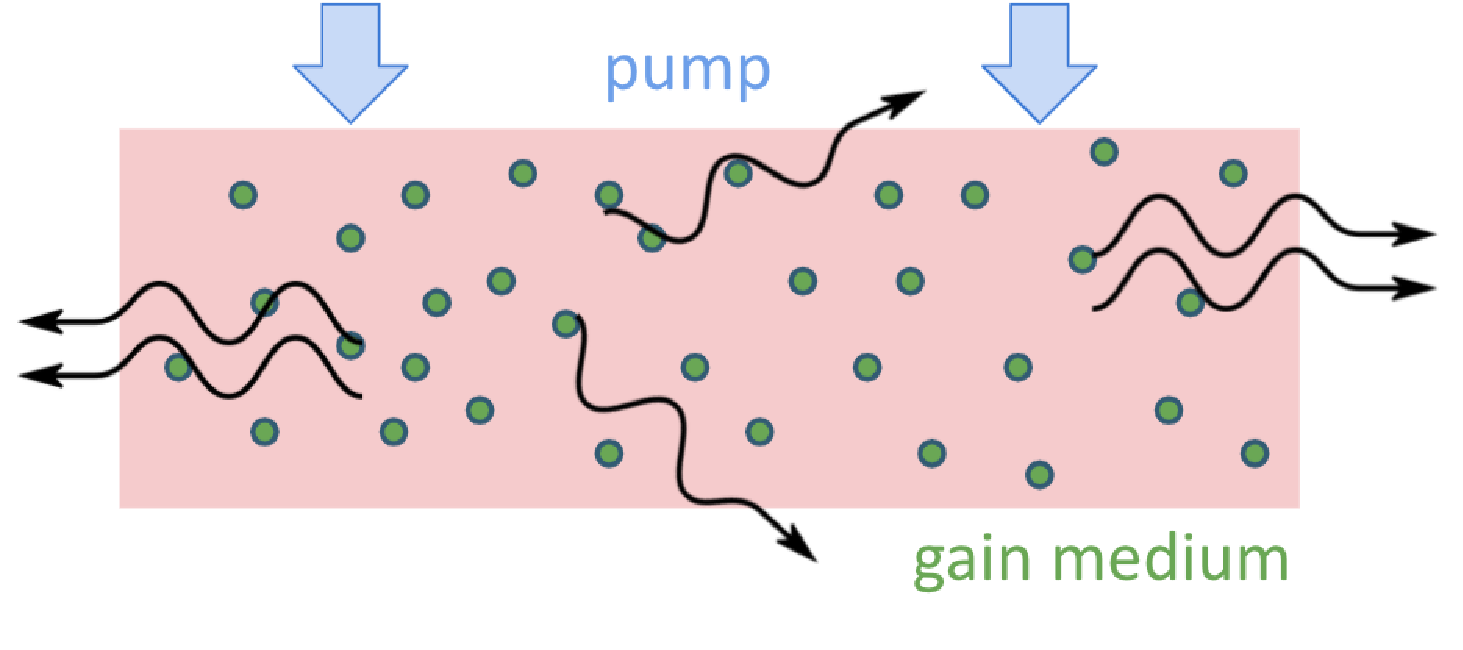
\includegraphics[width=0.5\textwidth]{lesson5/medium_pump.pdf}
    \label{図: 1}
    \caption{利得媒質+ポンプ}
\end{figure}
pumping lightを入れると、ある原子は励起状態になって、自然的に基底状態に戻り、光子が出てくる場合が多いですが、このままでは普通の光とあまり変わりがありません。そうすると、もっと強い光を入れる必要があります:
% medium + mirror
\begin{figure}[H]
    \centering
    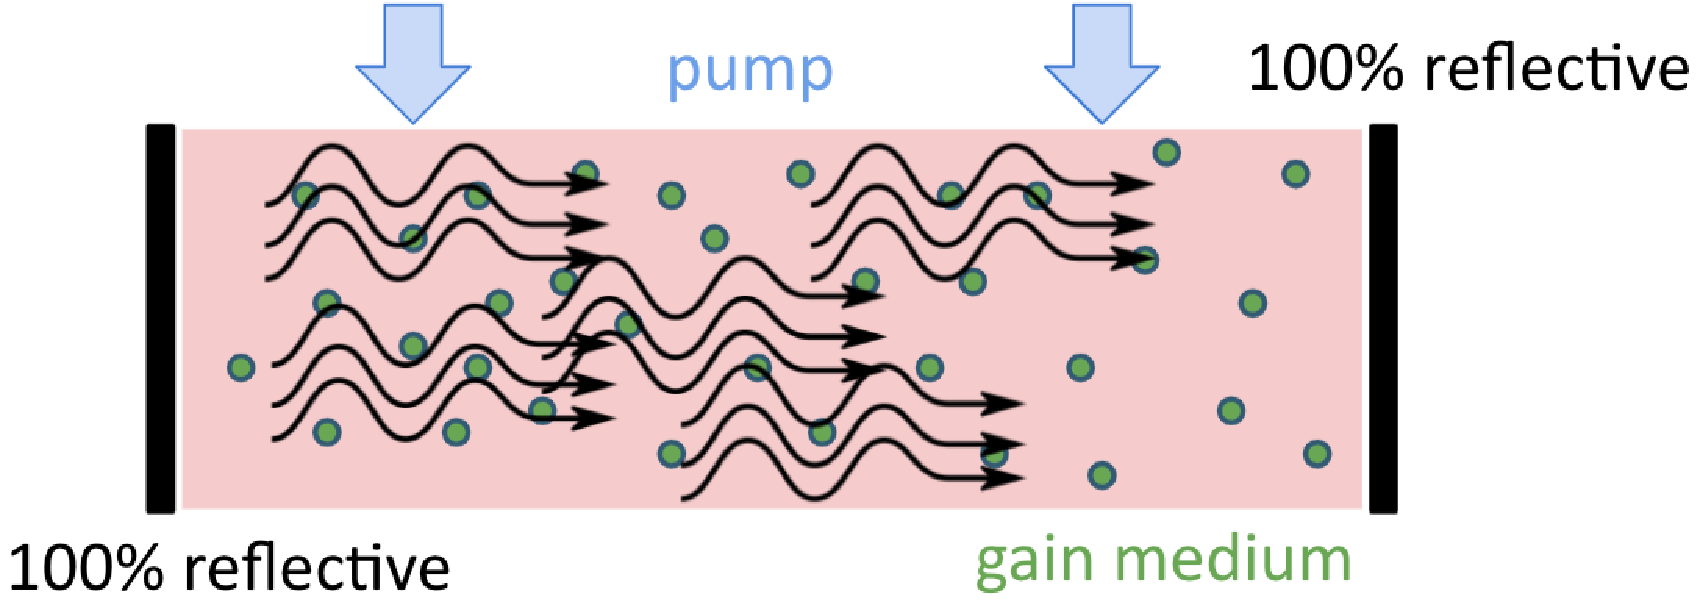
\includegraphics[width=0.5\textwidth]{lesson5/medium_mirrors.pdf}
    \label{図: 1}
    \caption{利得媒質+ポンプ+鏡}
\end{figure}
そこで、右側と左側に鏡をつけて、この媒質の中で光が反射します。光は繰り返し反射し続けて、上から入れているポンプの光と反射しているレーザーの光を合わせて、先程のエネルギーレベルの図のようなポンプの光とレーザーのエネルギーがあり、\textit{段々と各原子が放出する光子の、位相、波長、周波数が合ってきて、コヒーレントな状態}になっていきます。これを\textbf{カスケード効果}と言います。カスケードというのは滝という意味です。水がたくさん落ちてきているのと同じように、光がたくさん落ちてきているような状態です。こうすると、光はこの中で段々と強くなっていきます。

(この光を使うには)光を外に出さなければなりません。皆さんが見たことのあるレーザーは光が出てきていたと思います。どのように光を出すかというと、
(片方の)鏡を完璧な鏡ではなくて、例えば\textbf{99\%反射する鏡に変更}して、出てくる1\%の光も非常に強い光になります:
% medium + 99% mirror
\begin{figure}[H]
    \centering
    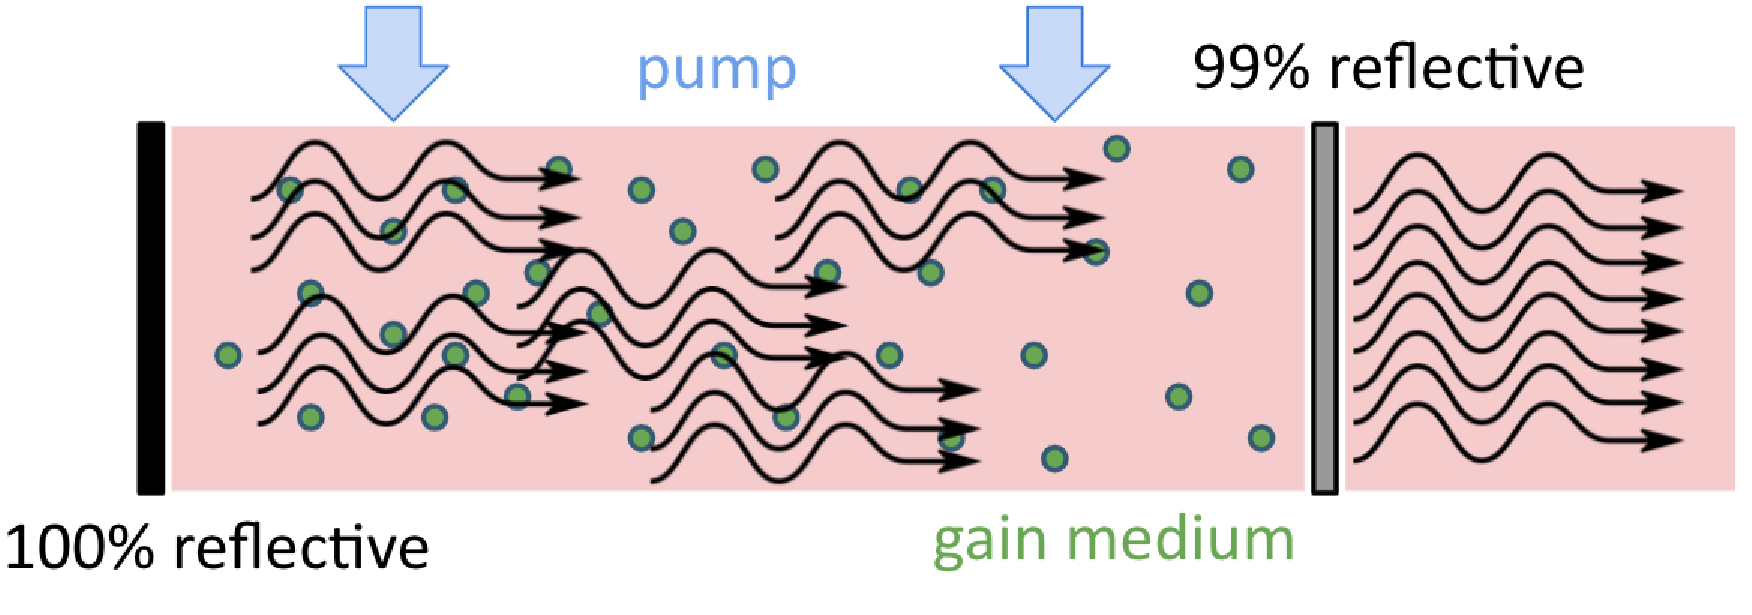
\includegraphics[width=0.5\textwidth]{lesson5/medium_99_mirror.pdf}
    \label{図: 1}
    \caption{利得媒質+ポンプ+99\%反射度鏡}
\end{figure}

99\%は中に残りますが、段々増幅され強い光となって、出てくる1%の光は十分強くて、コヒーレントな光になります。

\textbf{これを成功させるには、ポンプのレートはある閾値よりも大きくなくてはなりません}。そのような値をLasing threshold(レーザー閾値)と言います。
今まであまり数式は使いませんでしたが、少し数学的に見てみましょう:

$n(t)-$ number of photons

$N(t)-$ number of excited atoms

小文字の$n(t)$が光子の数で、大文字の$N(t)$が励起状態の原子の数であるとします。
\begin{equation}
\dot{n}=\operatorname{gain}-\text { loss }
\end{equation}
この$\Dot{n}$は光子の数の微分で、(gain - loss)でgainが何倍に増えて、lossが何倍に減っているかを表します。

gainの場合は、光子と励起状態の原子の両方が必要になります。このgainは$GnN$で表され、基本的にこの$G$ (gain coefficient) は0以上ですが、\textbf{1以上であれば強くなり、0から1の間であれば弱くなっていくということになります。}数式をもう一度書き直すと、gainの部分には$GnN$が入ります。lossについても見てみましょう。これは、鏡と鏡の間から逃げてしまう光子、上手く使えていない光子です。これは$kn$となり、$k$はloss coefficientで、常に0以上です。書き直すと、nの微分は$GnN - kn$になります:
\begin{equation}
\dot{n}=G n N-k n
\end{equation}
誘導放出が起こるとN(t)が減るので、ポンプの光を入れなければなりません。レーザーになっていない場合は、吸収と放出している光子の数は同じになるため、
大文字のN(t)は変わらず、$\Dot{n}=0$となり、$N(t) = N_0$となります。この落ち着いた(均衡した)状態が続きます。そうすると、$N(t)=N_0 - \alpha n$になり、この$\alpha$はStimulated Emission (誘導放出)となる比率です。

% insert non-linear, subbed in eqn
\begin{equation}
\dot{n}=\left(G N_{0}-k\right) n-(\alpha G) n^{2}
\end{equation}
これは非線形で、2乗の項を含んでいるため、(グラフは)パラボラの形状をしています。例を見てみましょう:

% insert non-positive parabola
\begin{figure}[H]
    \centering
    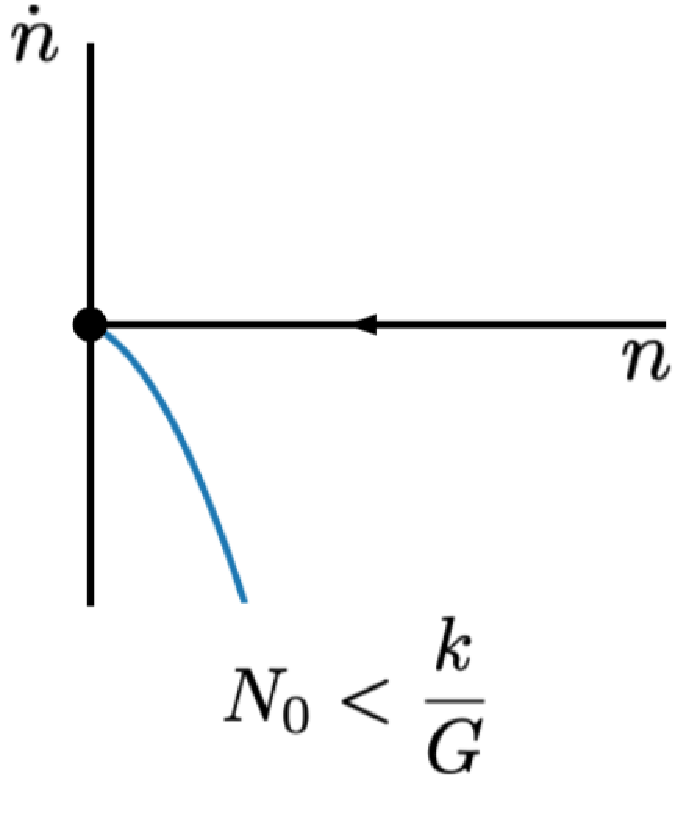
\includegraphics[width=0.5\textwidth]{lesson5/fully_negative_parabola.pdf}
    \label{図: 1}
    \caption{$N_0 < \frac{k}{G}$}
\end{figure}
縦軸は$\Dot{n}$(光子数の微分)で、横軸はnで励起状態にある原子の数を表します。基本的にどのような状態でも、右側にある物は左側に向かい、そのうち0に到達します。0に到達したら、$N_0$が続く状態であるので、ポンプの光を入れて、励起状態になり、それが落ちてくる確率が高いので、基本的に状態は変わらないです。

もっと強い光を入れると、$N_0$が大きくなって、カーブがこのようになります:
% insert downward parabola w/ positive component
\begin{figure}[H]
    \centering
    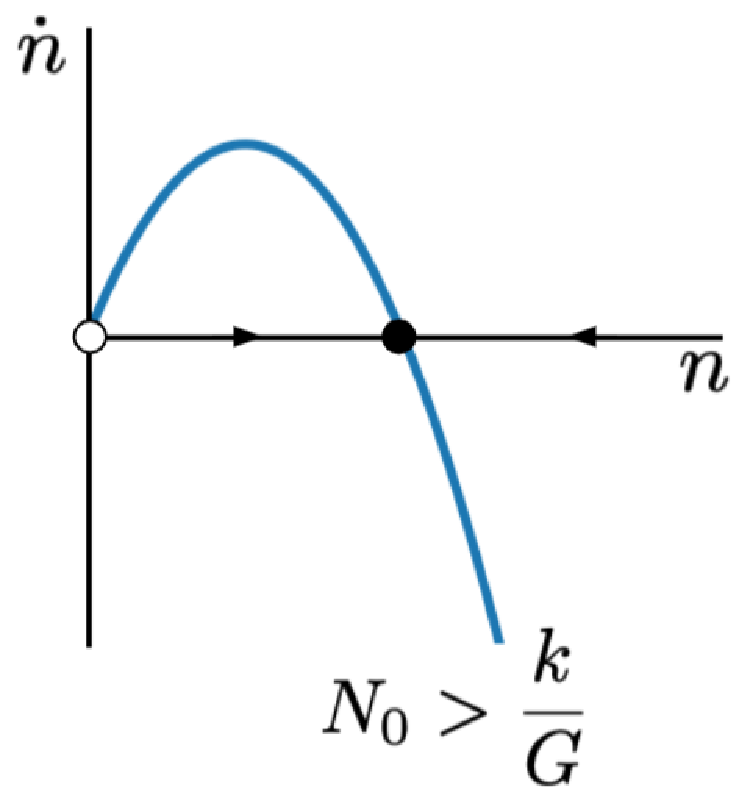
\includegraphics[width=0.5\textwidth]{lesson5/partially_negative_parabola.pdf}
    \label{図: 1}
    \caption{$N_0 > \frac{k}{G}$}
\end{figure}
これが$n^{2}$になっているため、このようなカーブになっています。このようなカーブでは、2箇所で$\Dot{n}$が0になっています。1つは、$N_0=\frac{k}{G}$という安定的な状態になっている時で、このような場合には、出てくる光と入っていく光は同じ大きさですが、真ん中(2つの0交点の間)にあると、出てくる光の方が強くなります。そうすると増幅の状態になります。

そのような非線形の状態で、先程のいくつかのパラメータにもよりますが、ポンプの光が弱い場合には、あまり面白い光の状態にはなりませんが、あるThreshold (閾値)よりも大きくなると、Amplification(増幅)の状態になります:
\begin{equation}
\dot{n}=\left(G N_{0}-k\right) n-(\alpha G) n^{2}
\end{equation}
% constant -> positive slope graph
\begin{figure}[H]
    \centering
    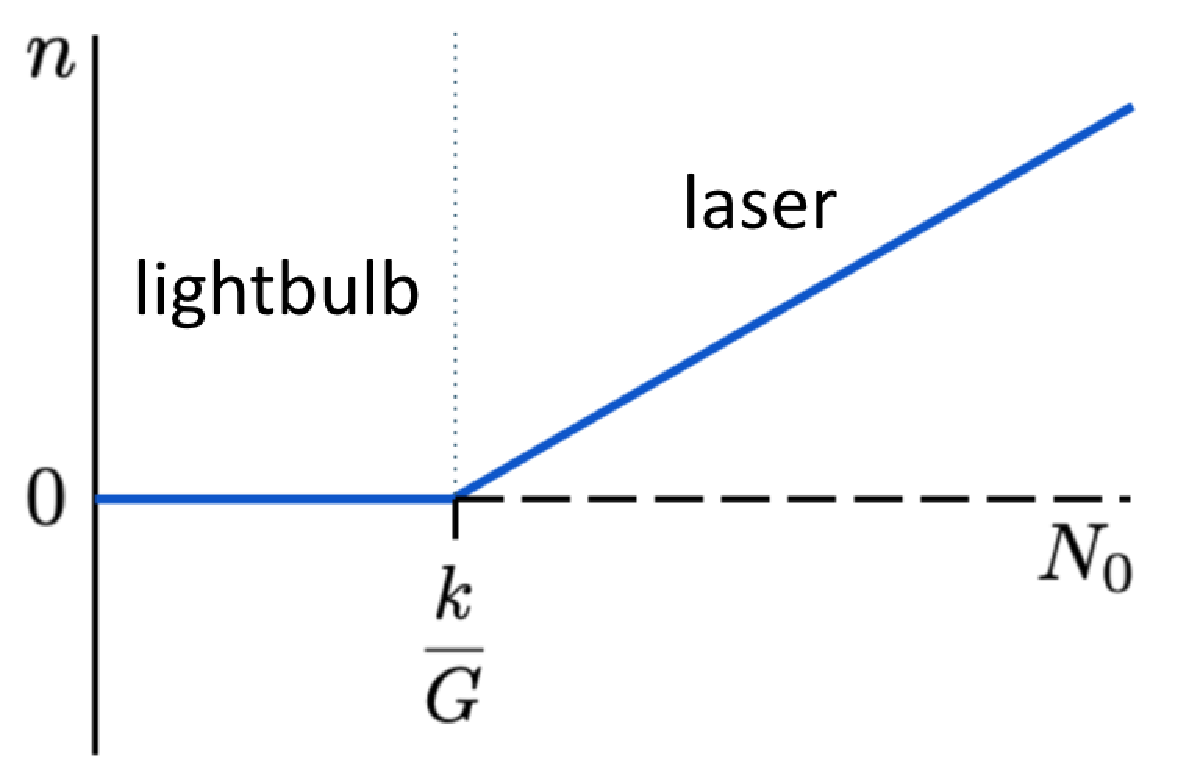
\includegraphics[width=0.5\textwidth]{lesson5/lightbulb_and_laser.pdf}
    \label{図: 1}
    \caption{電球とレーザのグラフ}
\end{figure}
それを\textbf{Lasing Threshold}と言います。左側は電球とあまり変わらず、右側に行くとLaserの状態になります。これは非常に突然起こるので、実験するとびっくりすると思います。レーザーは1958年に初めて発明され、これが初めて発見されました。



\section{単一光子}
古典通信では強い光を使いますが、沢山の光子を使ってそれ(情報)を1と0にエンコードします:
% 1/0 classical graph
\begin{figure}[H]
    \centering
    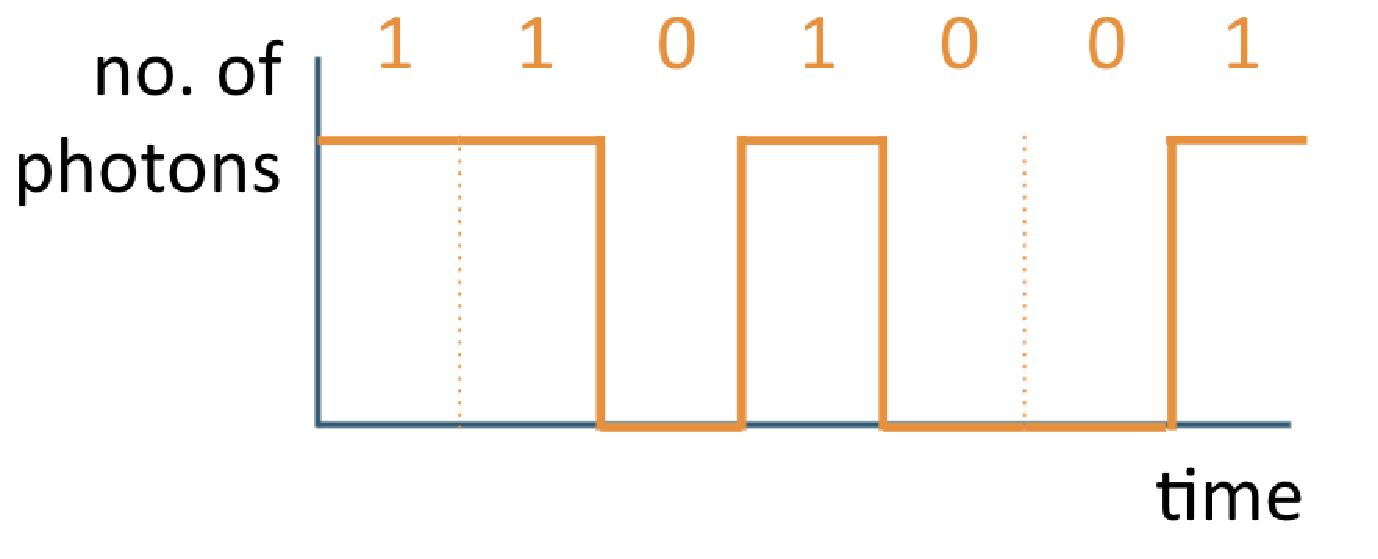
\includegraphics[width=0.5\textwidth]{lesson5/classical_encoding.pdf}
    \label{図: 1}
    \caption{古典通信符号化}
\end{figure}
例えば、光子が多い場合を1とエンコードし、光子があまりない場合を0にするというのがすごく基本的なエンコーディングですが、これは\textbf{ロバスト}で、(状態を)\textbf{作りやすい}し、\textbf{Amplification(増幅) も可能}で、 簡単に素早く作ることができます。\textbf{決定的} (Deterministic) にできるんですけれども問題は、\textbf{量子の場合にはあまり使えないことです}。量子の重ね合わせを全く作れないというわけではないですが、基本的に作れません。この授業では作れないという前提しましょう。これがエンタングル状態(を作るの)にも使えず、量子通信も得意ではないです。

そのため、単一の光子を使いたいです。
\subsection{減衰機を用いる単一光子を作る手法}
% laser + attenuators
\begin{figure}[H]
    \centering
    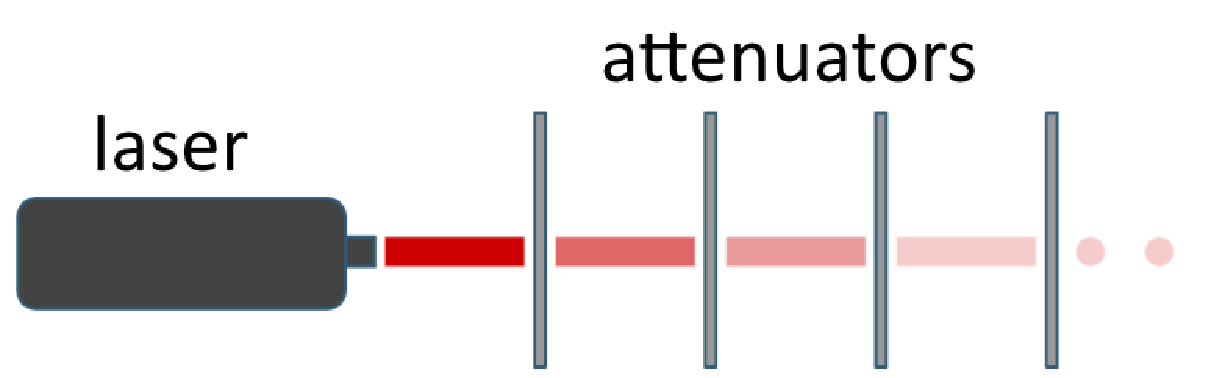
\includegraphics[width=0.5\textwidth]{lesson5/laser_attenuator.pdf}
    \label{図: 1}
    \caption{減衰機とレーザーの系}
\end{figure}
単一の光子は量子状態を持ち、理想的には先程説明したレーザーを使って、(その光を)だんだん弱めていくことで取り出すことができ、減衰機(attenuator)を連続でかけて、例えば
1つ(の減衰機)毎に10\%しか通さないとすると、$\frac{1}{10}$, $\frac{1}{100}$, $\frac{1}{1000}$, $\frac{1}{10000}$となり、最終的には1個ずつの光子が出てきます。これは、光がそのような量子状態を持っていることを証明する実験などには使えますが、光子が1つ残るのか、2つ残るのか、残らないのかというのは、確率的で、通信としてはあまり実用的ではありません。
これが\textit{ポアソン分布}(に従うの)ですが、\textit{各光子がいつ入ってくるか、本当に入ってくるかどうか、放出できているかどうか証明しにくいので使いにくいです。
}この量子状態は量子通信にはあまり実用的ではありません。では、(量子通信に必要な状態は)どのように作れるでしょうか?


\subsection{Heraldを用いる単一光子を作る手法}
まずは\textbf{herald}ということについてみていきます。heraldというのは、光子を一つ作ったか、作っていないかという情報になります:
% herald pic
\begin{figure}[H]
    \centering
    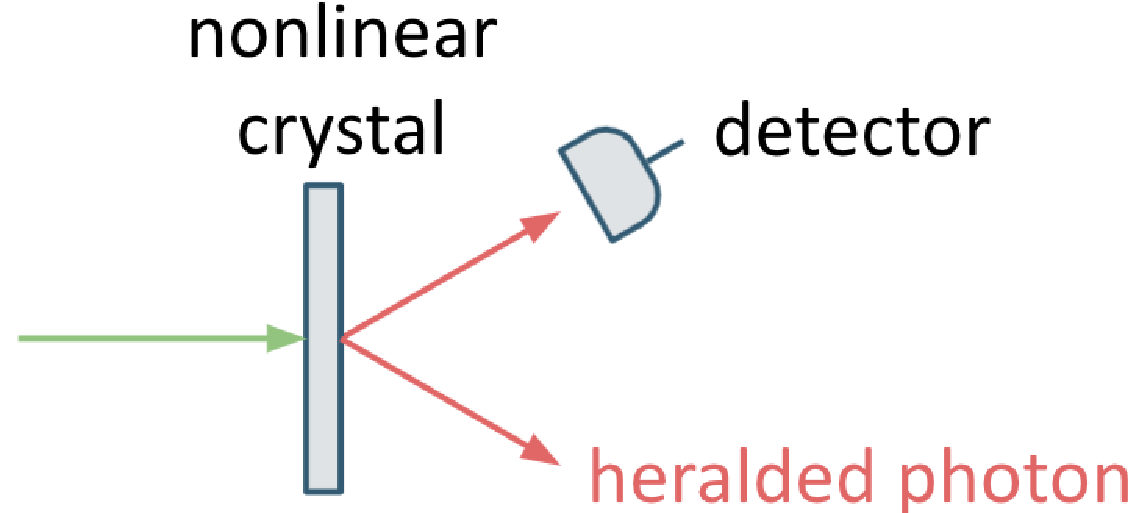
\includegraphics[width=0.5\textwidth]{lesson5/heralding.pdf}
    \label{図: 1}
    \caption{Heraldingの図}
\end{figure}

例えば2つの光子を作ったら、(その内)一つは光子のペアを作りましたという証明になります。これは前に説明したSPDCの手法で、強い光を入れて時々Entangleされている二つの光子が出てきます。一つはdetect(観測)して、一つの光子が測定されるときには、もう一つの光子が光子が生成できているということになります。決まった方向に(光子が)行くため、うまくフィルタリングすることで、もう一つの単一光子を使うことができます。いくつかの問題があります:
\begin{itemize}
    \item 測定器が実際には測定していないにも関わらず、測定したというように判定してしまうこと
    \item 当たっててもクリック(測定)しないこともあります。
    \item これはまだ確率的なプロセスで、$10^{-8}$くらいの確率であるため、いつ単一光子が得られるのかはわかりません。
\end{itemize}
\subsection{決定的に単一光子を作る手法}
決定的に単一光子を作ることはできるでしょうか?いくつかの手法が提案されていますが、完璧な単一光子を作る手法はまだありません。
% 3 stage atom w/ annotations
\begin{figure}[H]
    \centering
    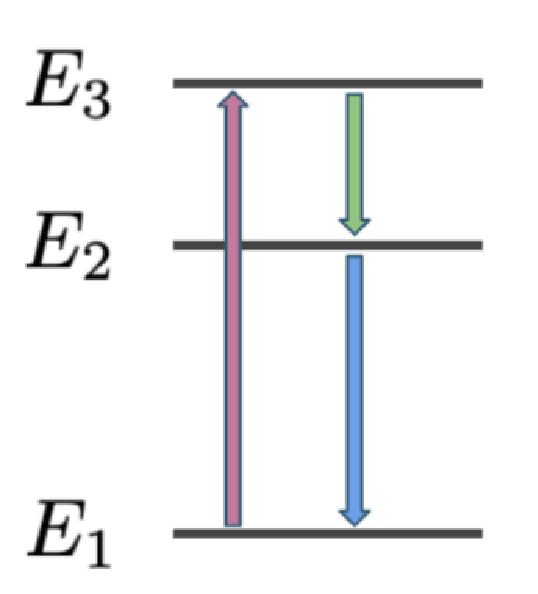
\includegraphics[width=0.5\textwidth]{lesson5/3_stage_arrows.pdf}
    \label{図: 1}
    \caption{3エネルギーレベルシステム}
\end{figure}
一つの例としては、これはレーザーに近い手法ですが、3つの(エネルギー)レベルのシステムを使って:
\begin{enumerate}
    \item $E_1$から$E_3$の励起状態を作り
    \item $E_3$から$E_2$に自然に落ち
    \item 最後に$E_2$から$E_1$に落ちる誘導放出を制御できれば、光子がいつ出てくるのかを制御できるようになります。
\end{enumerate}
これは、\textbf{$E_2$のStability (安定性)次第になります}。このような材料が世の中にはあるのでしょうか?

一つの例としては\textbf{Nitrogen vacancy (center in ) diamond}というものです。
% NV diamond (Source: NIST)
\begin{figure}[H]
    \centering
    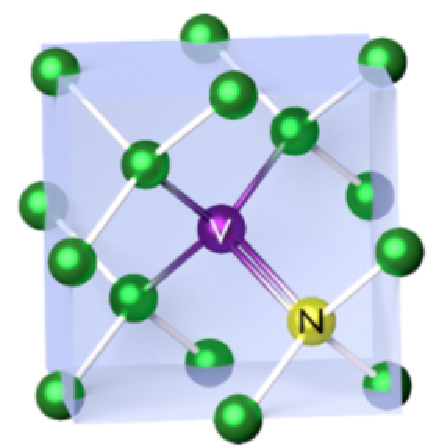
\includegraphics[width=0.4\textwidth]{lesson5/NV_Diamond.pdf}
    \label{図: 1}
    \caption{diamond中のNV中心・参考資料:NIST}
\end{figure}
量子通信ではよく出てくる物質で、炭素の原子がdiamondの形になっており、一つの炭素原子だけ抜いて、そこが空洞になりますが、そこにNitrogen(窒素)を入れて、結晶の形が変わり、その部分をうまく使うことで、電子一つを保存することができ、その電子をうまく使えば、このようなシステムを作ることができるかもしれません。

これはさまざまな特徴を持っているため、量子通信では非常によく使われる材料になります。以上が単一光子に関してです。この先も単一光子についての話が出てきますが、今回はここまでにしましょう。


